\documentclass[12pt]{elsarticle}

\usepackage{amssymb}
\usepackage{lineno}

\journal{}

\begin{document}
	
	\begin{frontmatter}
		
		%% Title, authors and addresses
		
		%% use the tnoteref command within \title for footnotes;
		%% use the tnotetext command for the associated footnote;
		%% use the fnref command within \author or \address for footnotes;
		%% use the fntext command for the associated footnote;
		%% use the corref command within \author for corresponding author footnotes;
		%% use the cortext command for the associated footnote;
		%% use the ead command for the email address,
		%% and the form \ead[url] for the home page:
		%%
		%% \title{Title\tnoteref{label1}}
		%% \tnotetext[label1]{}
		%% \author{Name\corref{cor1}\fnref{label2}}
		%% \ead{email address}
		%% \ead[url]{home page}
		%% \fntext[label2]{}
		%% \cortext[cor1]{}
		%% \address{Address\fnref{label3}}
		%% \fntext[label3]{}
		
		\title{Solution of the Incompressible Navier-Stokes Equations using Finite Volume Methods}
		
		
		
		%% use optional labels to link authors explicitly to addresses:
		%% \author[label1,label2]{<author name>}
		%% \address[label1]{<address>}
		%% \address[label2]{<address>}
		
		\author{Karthik Reddy Lyathakula}
		
		\address{North Carolina State University, Raleigh,  United States}
		
	\end{frontmatter}
	
	%%
	%% Start line numbering here if you want
	%%
	%%\linenumbers
	
	%% main text
	\section{Introduction}
	\label{S:1}
	
	The incompressible Navier stokes(INS) equation is a mixed hyperbolic/ elliptical in time. To solve this system, the equations are split so that the elliptical part is separated from the hyperbolic part. There are two methods for splitting the equation:
	
	\begin{enumerate}
		\item Artificial compressibility(AC) form
		\item projection form
	\end{enumerate}
	
	In this project, the AC method is used to solve the incompressible Navier stokes equation. Further, the AC method is extended to immersed boundary methods.
	
	\begin{figure}[h]
		\centering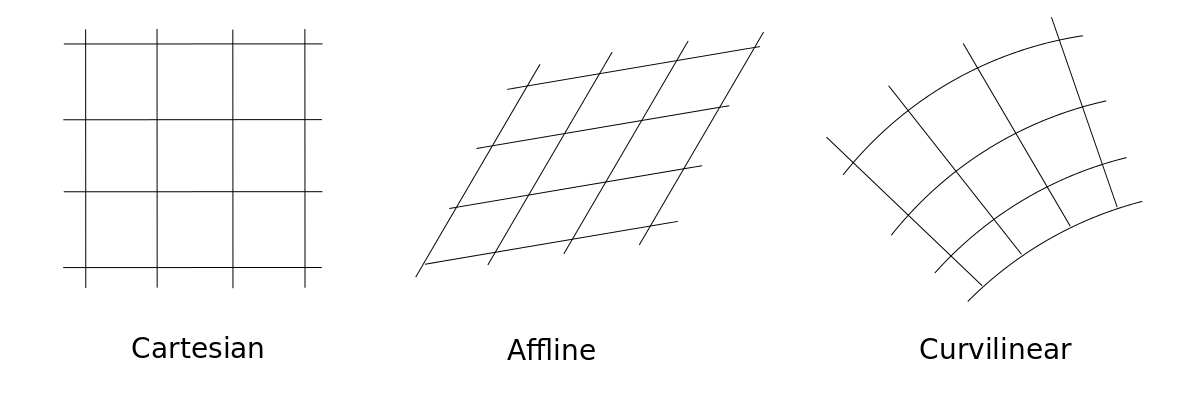
\includegraphics[width=1\linewidth]{finite_difference_grids.png}
		\caption{Different types of meshes}
	\end{figure}
	
	\section{Artificial compressiblity method}
	\label{S:2}
	In this section, artificial compressibility method to solve INS equation is discussed. The INS equation in AC form is shown below:
	
	\begin{equation}
		\frac{1}{\beta^2}\frac{\partial p}{\partial t}+\bigtriangledown \cdot(\rho \overrightarrow{u})=0
	\end{equation}
	
	\begin{equation}
		\frac{\partial (\rho \overrightarrow{u})}{\partial t}+\bigtriangledown \cdot (\rho \overrightarrow{u} \overrightarrow{u})+\bigtriangledown p -\bigtriangledown \cdot \mu \bigtriangledown \overrightarrow{u} =0
	\end{equation}
	here $\beta$ is the speed of sound. The INS equation is discretized by integrating the equation with respect to volume and applying gauss divergence theorem to convert the volume integral to surface integral as shown below`:
	
	\begin{equation}
		\int_V \bigtriangledown \cdot  \bigtriangledown \phi \,dV 
	\end{equation}\newline
	
	\begin{equation}
		\oint_S \bigtriangledown \phi \cdot n \,dA 
	\end{equation}
	
	To solve above equation over the required domain, the domain is divided into infinitesimal volumes called mesh elements. Few examples of meshes are shown in figure 1. The INS is approximated on each cell center as follows:
	
	\begin{equation}
		\frac{\partial (\rho \overrightarrow{u})}{\partial t}+\sum\limits_{k=1}^N \rho (\overrightarrow{u} \cdot \overrightarrow{n}) A_k=0
	\end{equation}
	\begin{equation}
		\frac{\partial (\rho \overrightarrow{u})}{\partial t}+\sum\limits_{k=1}^N \rho \overrightarrow{u} (\overrightarrow{u} \cdot \overrightarrow{n}) A_k+\sum\limits_{k=1}^N p \overrightarrow{n}-\mu \bigtriangledown \overrightarrow{u}=0
	\end{equation}
	
	Here $\overrightarrow n$ is the outward normal. In this project, quadrilateral mesh will be used and the value of N will be 4. By applying above equation on a cell (i,j) as shown in the figure2, they give rise to mass and momentum fluxes on the cell face. They can be represented as:
	
	\begin{figure}[h]
		\centering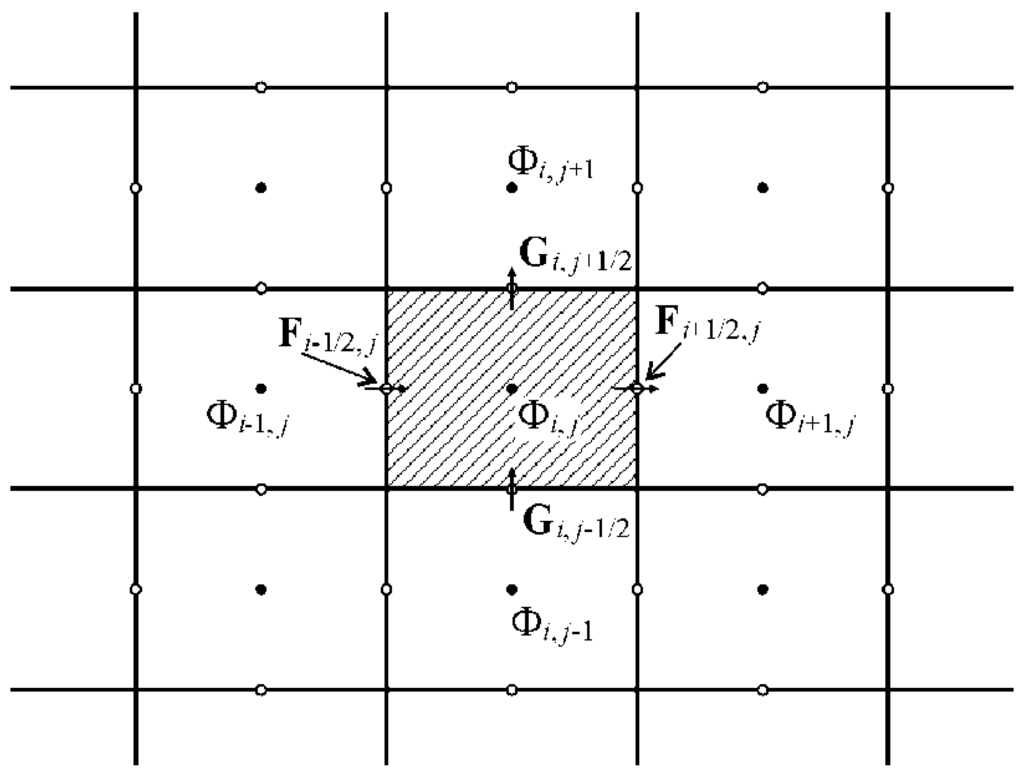
\includegraphics[width=0.8\linewidth]{phi_grid.png}
		\caption{Different types of meshes}
	\end{figure}
	
	\begin{equation}
		F_{i+\frac{i}{2},j}-F_{i-\frac{i}{2},j}+G_{i,j+\frac{i}{2}}-G_{i,j--\frac{i}{2}}
	\end{equation}
	Here F and G are the fluxes in x and y directions respectively. In INS, there are inviscid fluxes and viscous fluxes. Viscous fluxes are computed using different methods (shown below) which are implemented and tested on a poisons equation in project 2. .
	
	\begin{enumerate}
		\item Parallel CV method
		\item Thin layer method
		\item Tangent / normal gradient decomposition method
	\end{enumerate}
	
	The inviscid terms of the momentum equation and mass fluxes are calculated by summation over the faces. In this work, the field variables are stored at the cell centers and this causes spurious oscillations due to central difference schemes. To avoid it, dissipative terms are added to the mass flux calculation, according to Rhie-chow criteria, on each cell face as shown below:
	
	\begin{equation}
		massflux_{i+1/2,j}= (\rho \overrightarrow{u} \cdot \overrightarrow{n})_{i+1/2,j} +f* (P_L-P_R)
	\end{equation} 
	Here f is calculated from Eigen value analysis of the INS system and it is given by:
	
	\begin{equation}
		\lambda_{max}=0.5*(\overrightarrow{u} \cdot \overrightarrow{n})+0.5*\sqrt{(\overrightarrow{u} \cdot \overrightarrow{n})+4*\beta_{i+1/2,j}^2} 
	\end{equation}
	\begin{equation}
		f=const*\frac{\lambda_{max}}{\beta_{i+1/2,j}^2} 
	\end{equation}
	There are different method to calculate $P_L$ $P_R$ like linear method, higher order method. In linear method $P_L =p_{i-1,j}$ $P_R=p_{i+1,j}$ is used. For higher order:
	
	\begin{equation}
		P_L=p_i+0.5*avg(p_{i+1}-p_i,p_i,p_{i-1})
	\end{equation}
	\begin{equation}
		P_R=p_i-0.5*avg(p_{i+1}-p_i,p_{i+2},p_{i+1})
	\end{equation}
	Here avg is the operator that can be calculated in number of different ways. In this project TVD criteria will be used and as per TVD, avg operator is calculated as:
	
	\begin{equation}
		avg(a,b)=0.5*(sign(a)+sign(b))min(abs(a),abs(b)
	\end{equation}
	
	The next important criteria for the simulation is selection of time step. In this project, two time stepping are used. One is the local time stepping which is calculated in each cell based on the maximum Eigen value and the second is global time step, which is the minimum of local time step.
	
	
	\section{Results}
	Incompressible Navier stokes equation using artificial compressibility method is solved to capture flow inside a lid-driven cavity and flow through two different channels for various Reynolds numbers. For this project, a C++ program with various subroutines is used to solve the flow equations, and Tecplot, MATLAB is used for plotting the results. The code is attached to the appendix.\\
	
	\begin{figure}[h]
		\caption{Square Grid 50x50}
		\centering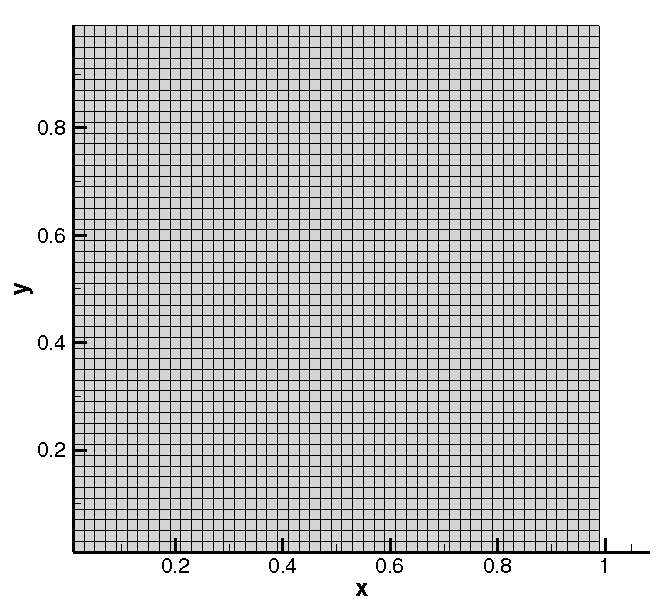
\includegraphics[width=0.7\linewidth]{grid_50_50.png}
		\caption{Square Grid 100x100}
		\centering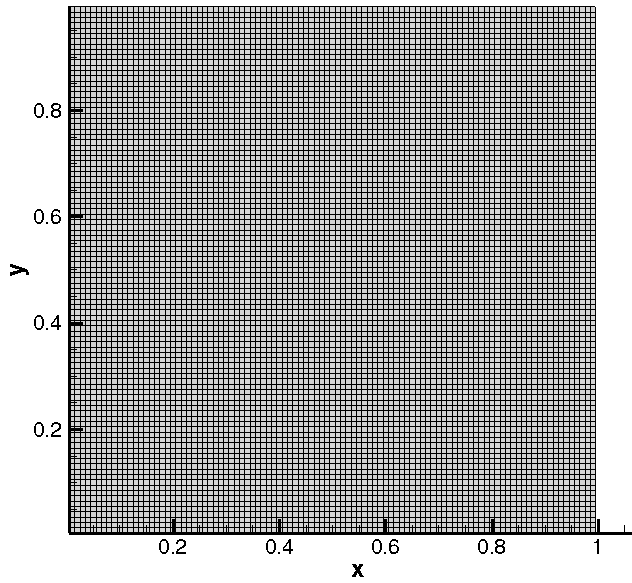
\includegraphics[width=0.7\linewidth]{grid_100_100.png}
	\end{figure}
	\clearpage
	
	\begin{figure}[h]
		\caption{grid3}
		\centering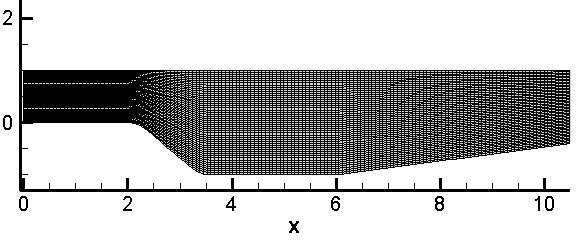
\includegraphics[width=0.7\linewidth]{grid3}
		\caption{grid4}
		\centering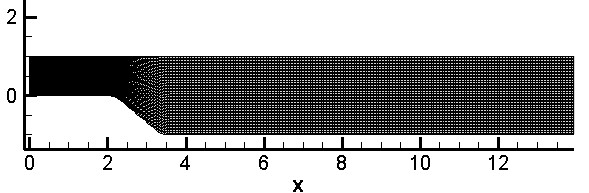
\includegraphics[width=0.7\linewidth]{grid4}
	\end{figure}
	
	\subsection{Lid Driven Cavity}
	
	The lid-driven cavity is a classical problem, where the top wall of a closed square chamber is moving in the tangential direction with a certain velocity, and flow inside the chamber is captured for different Reynolds numbers. The Reynolds number for this problem is defined as:
	
	\begin{equation}
		Re=\frac{\rho U L}{\mu}
	\end{equation}
	here $\rho$ is the density of the fluid, $U_{wall}$ is the wall velocity, L is the length of the square cavity and $\mu$ is the viscosity of the fluid. The Reynolds for the problem is changed by decreasing the viscosity and using the same values for the rest of the parameters. For the simulation, a relative tolerance of 1e-4 is taken for momentum residue to converge and it is found that mass residue is 1e-21, which is negligible.  \newline
	\newline
	Figures. \ref{start:50x50_RE:100}- \ref{End:50x50_RE:100} shows the results for Re=100 on grids 50x50 and 100x100 using linear approximation, TVD approximation for the Rhi-chow interpretation.\newline
	\newline
	Fig. 7, 8 shows the velocity magnitude contours for linear,  TVD approximation respectively and Fig.9 ,10 shows the comparison of velocities through geometric centers with reference values(Ghia et. al). It can be observed that there is a slight difference in the contour profiles and this difference can be observed from the 1d plots. By using TVD approximation, the results are improved slightly compared to linear approximation. Fig. 11, 12 shows the logarithmic values of residues with iteration number and it can be observed that the number of iterations required to converge using TVD is more than a linear approximation. \newline
	\newline
	The flow is also solved for Re=100 on a 100x100 grid and Fig. 13 - Fig. 18 shows the results for this case. The results follow a similar trend as that of the 50x50 grid.  Fig 19-22 shows the mesh refinement effect on the flow velocities. It can be observed that the 100x100 mesh is showing better results than the 50x50 grid. Also, the number of iterations required for converging with 100x100 grid is more as the absolute residue is going lower than 50x50 grid and hence 100x100 grid is more accurate. Fig. 23, 24 shows the vorticity and streamlines respectively. It can be observed that there is a small recirculation at the bottom right corner of the lid-driven cavity. 
	
	\begin{figure}[h]
		\caption{Velocity magnitude with RE=100 and 50x50 grid using linear approximation}
		\centering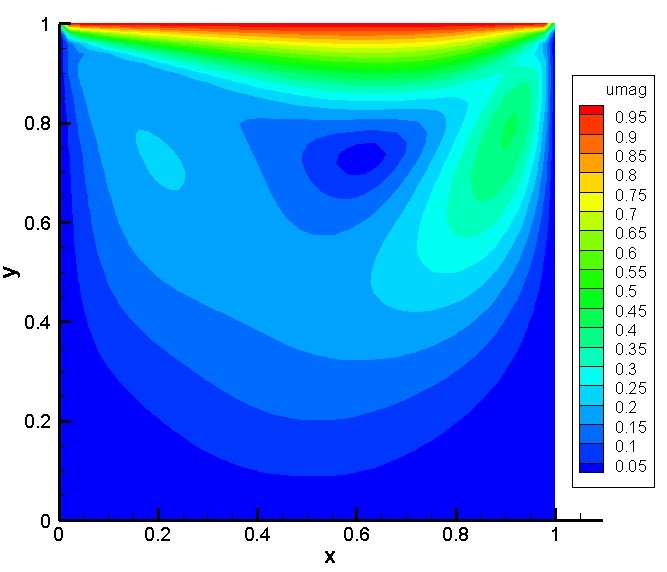
\includegraphics[width=0.8\linewidth]{1_50_50_re_100_velocity_linear}
		\label{start:50x50_RE:100}
		\caption{Velocity magnitude with RE=100 and 50x50 grid using TVD approximation}
		\centering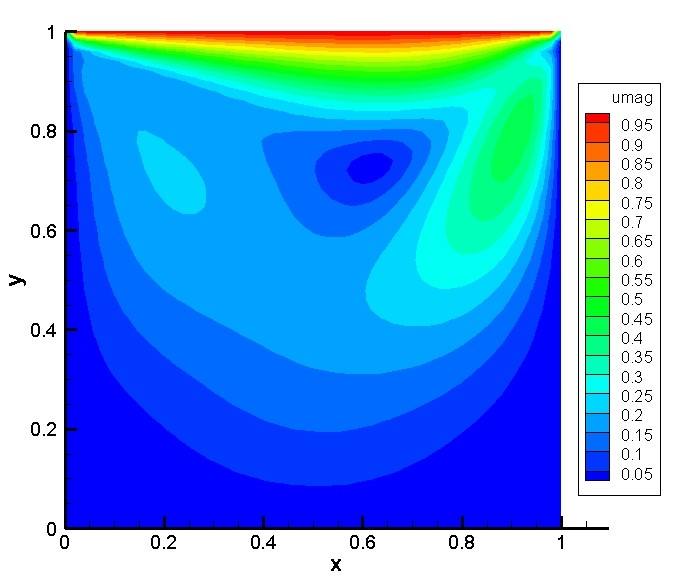
\includegraphics[width=0.8\linewidth]{2_50_50_re_100_velocity_tvd}
	\end{figure}
	
	\begin{figure}[h]
		\caption{Comparison of u velocities}
		\centering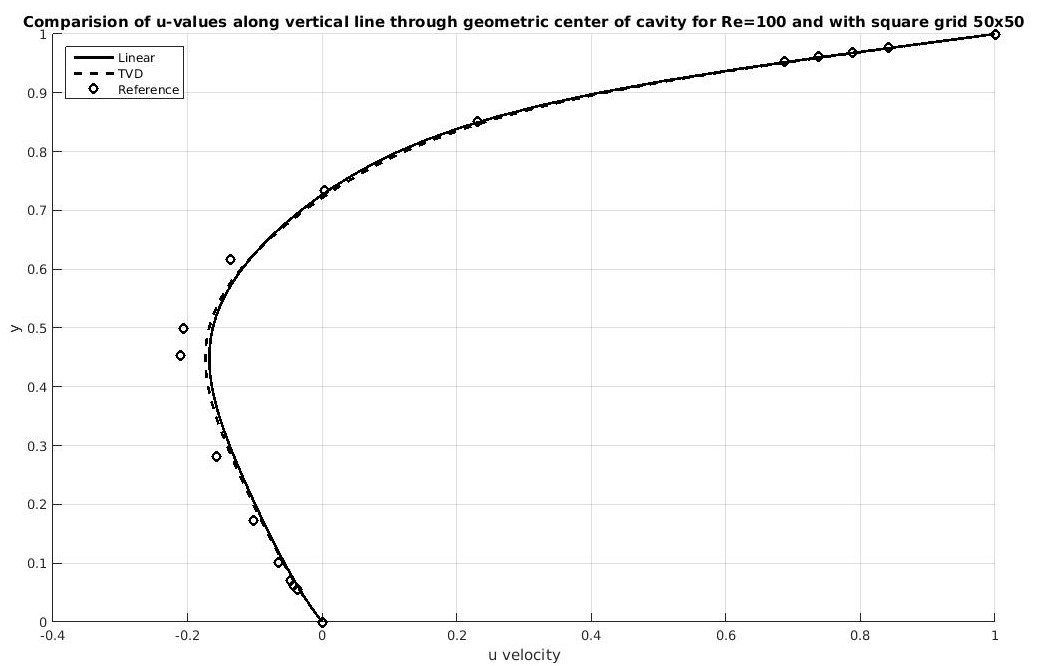
\includegraphics[width=1.0\linewidth]{5_uvalues_tvd_linear_re_100_50_50}
		\caption{Comparison of v velocities}
		\centering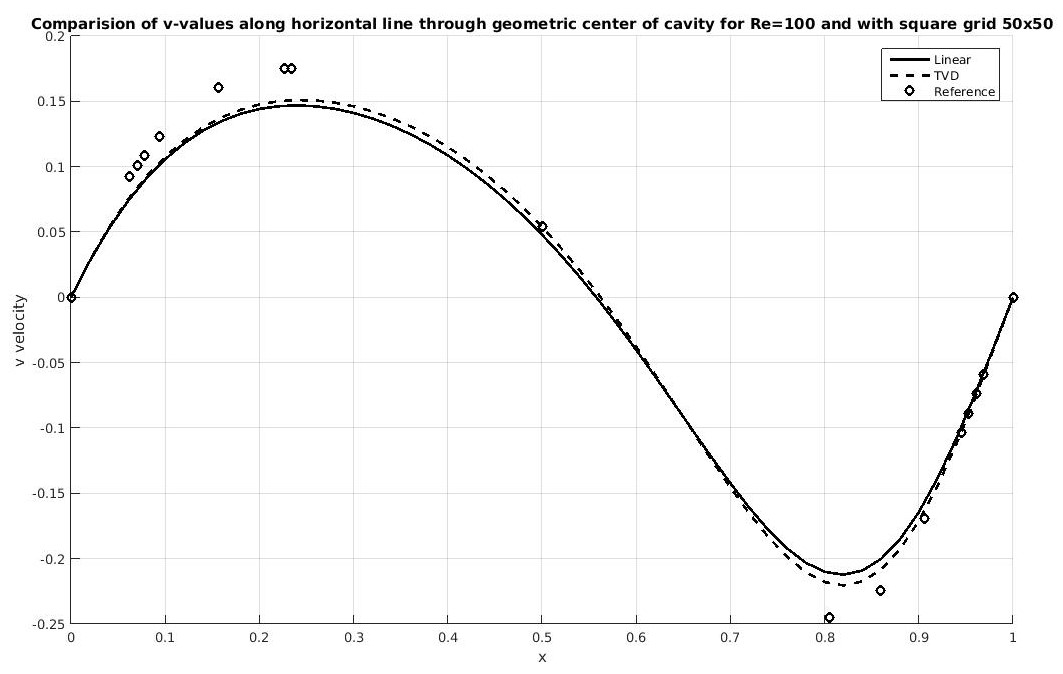
\includegraphics[width=1.0\linewidth]{6_vvalues_tvd_linear_re_100_50_50}
	\end{figure}
	
	\begin{figure}[h]
		\caption{Comparison of Relative Residue}
		\centering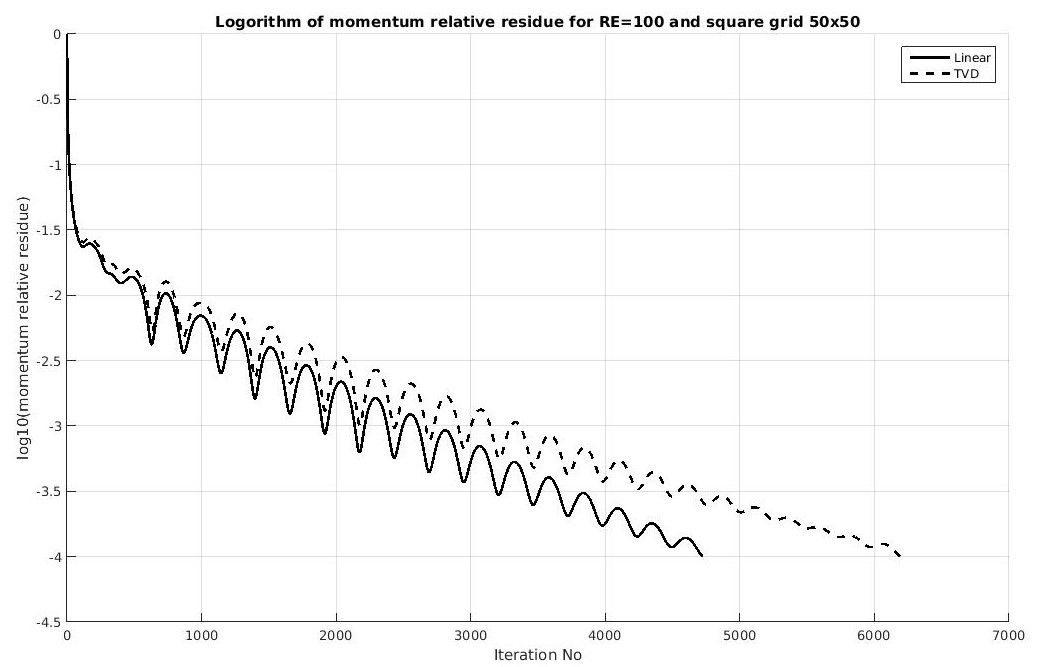
\includegraphics[width=1.0\linewidth]{3_rr_tvd_linear_re_100_50_50}
		\caption{Comparison of Absolute Residue}
		\centering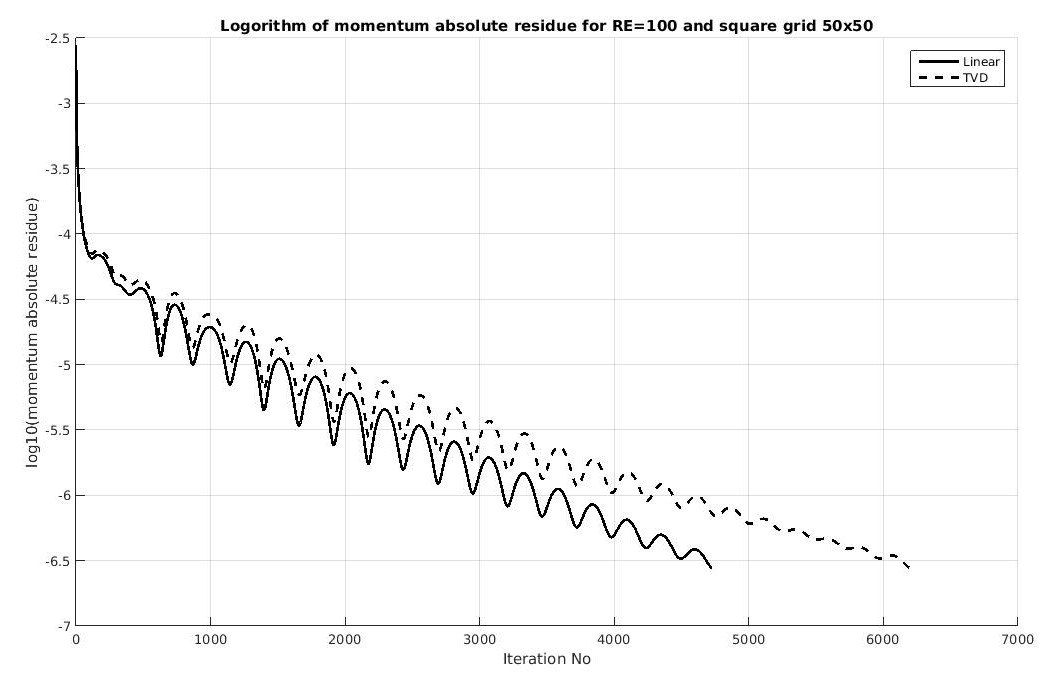
\includegraphics[width=1.0\linewidth]{4_ar_tvd_linear_re_100_50_50}
	\end{figure}
	\clearpage
	
	\begin{figure}[h]
		\caption{Velocity magnitude with RE=100 and 100x100 grid using linear approximation. }
		\centering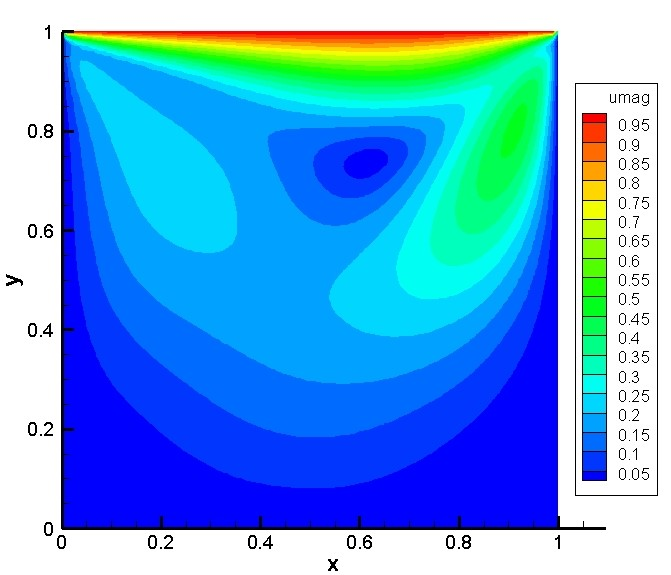
\includegraphics[width=0.9\linewidth]{7_100_100_re_100_velocity_linear}
		\caption{Velocity magnitude with RE=100 and 00x100 grid using TVD approximation. }
		\centering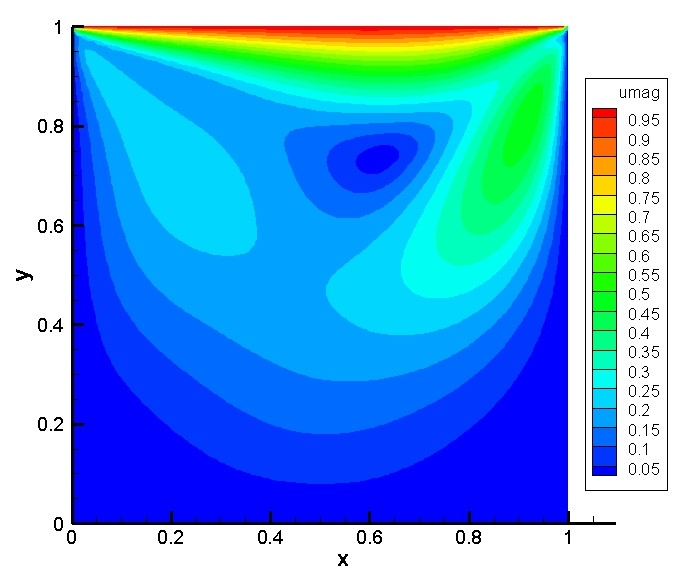
\includegraphics[width=0.9\linewidth]{8_100_100_re_100_velocity_tvd}
	\end{figure}
	
	\begin{figure}[h]
		\caption{Comparison of u velocities}
		\centering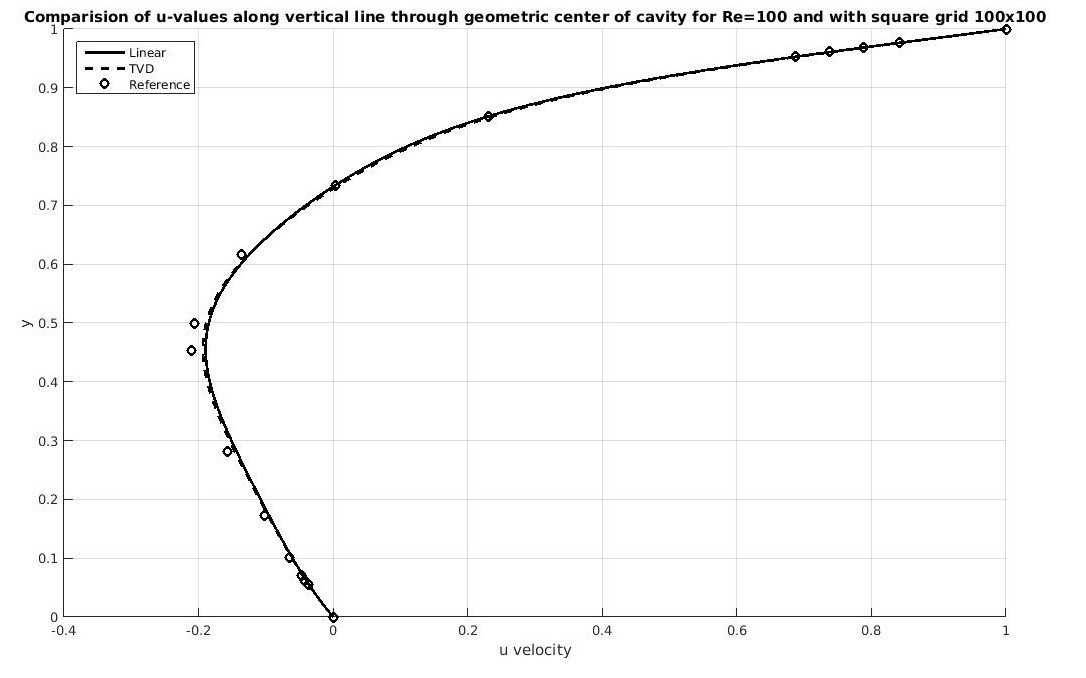
\includegraphics[width=1.0\linewidth]{11_uvalues_tvd_linear_re_100_100_100}
		\caption{Comparison of v velocities}
		\centering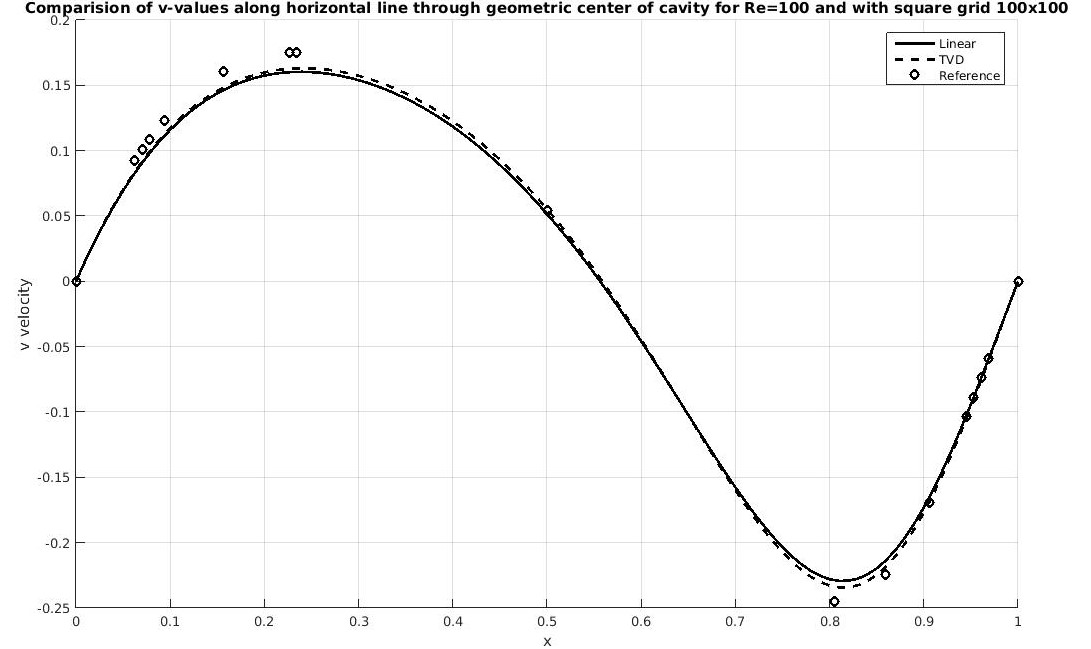
\includegraphics[width=1.0\linewidth]{12_vvalues_tvd_linear_re_100_100_100}
	\end{figure}
	
	
	\begin{figure}[h]
		\caption{Comparison of Relative Residue}
		\centering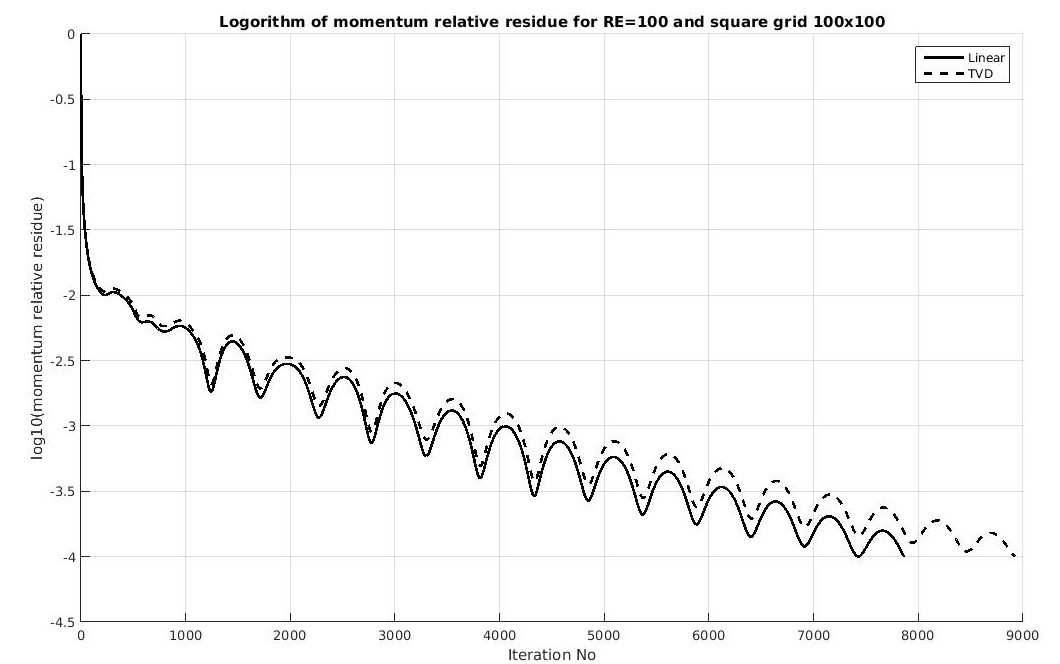
\includegraphics[width=1.0\linewidth]{9_rr_linear_re_100_100_100}
		\caption{Comparison of Absolute Residue}
		\centering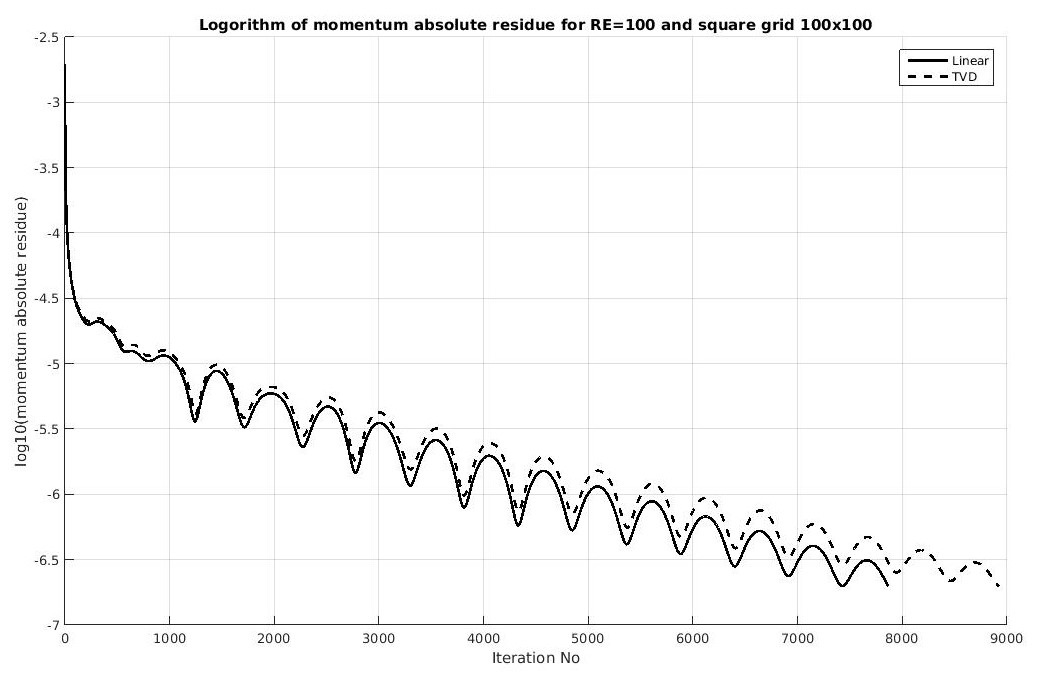
\includegraphics[width=1.0\linewidth]{10_ar_linear_re_100_100_100}
	\end{figure}
	
	\begin{figure}[h]
		\caption{Effect of mesh refinement on u velocities}
		\centering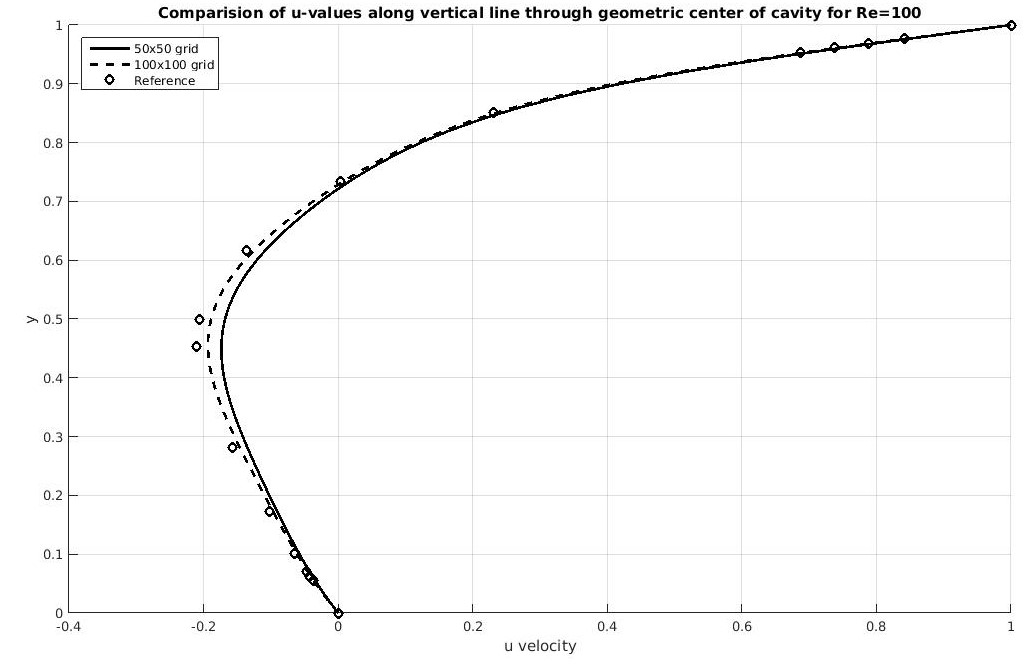
\includegraphics[width=1.0\linewidth]{15_uvel_mesh_comparision}
		\caption{Effect of mesh refinement on v velocities}
		\centering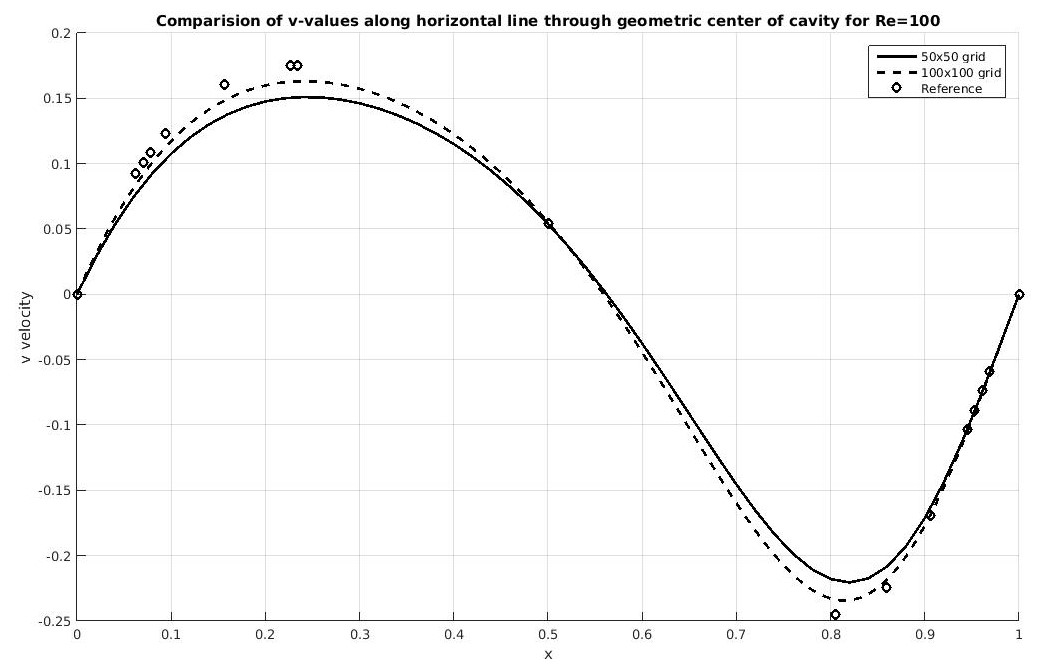
\includegraphics[width=1.0\linewidth]{16_vvel_mesh_comparision}
	\end{figure}
	
	\begin{figure}[h]
		\caption{Effect of mesh refinement on Relative Residue}
		\centering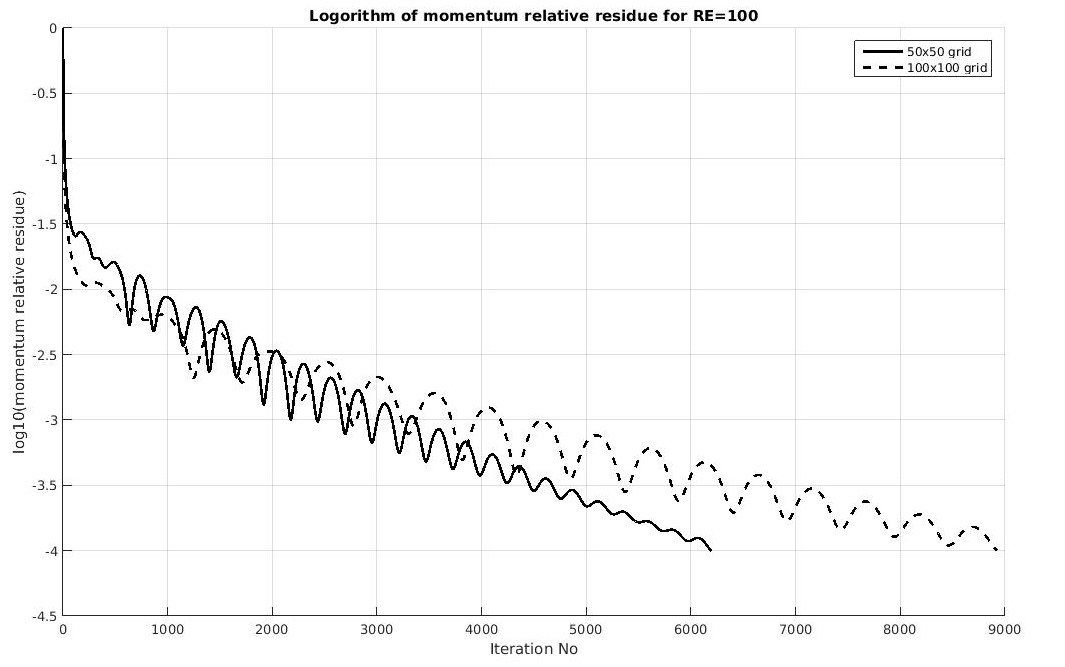
\includegraphics[width=1.0\linewidth]{13rr_mesh_comparision}
		\caption{Effect of mesh refinement on Absolute Residue}
		\centering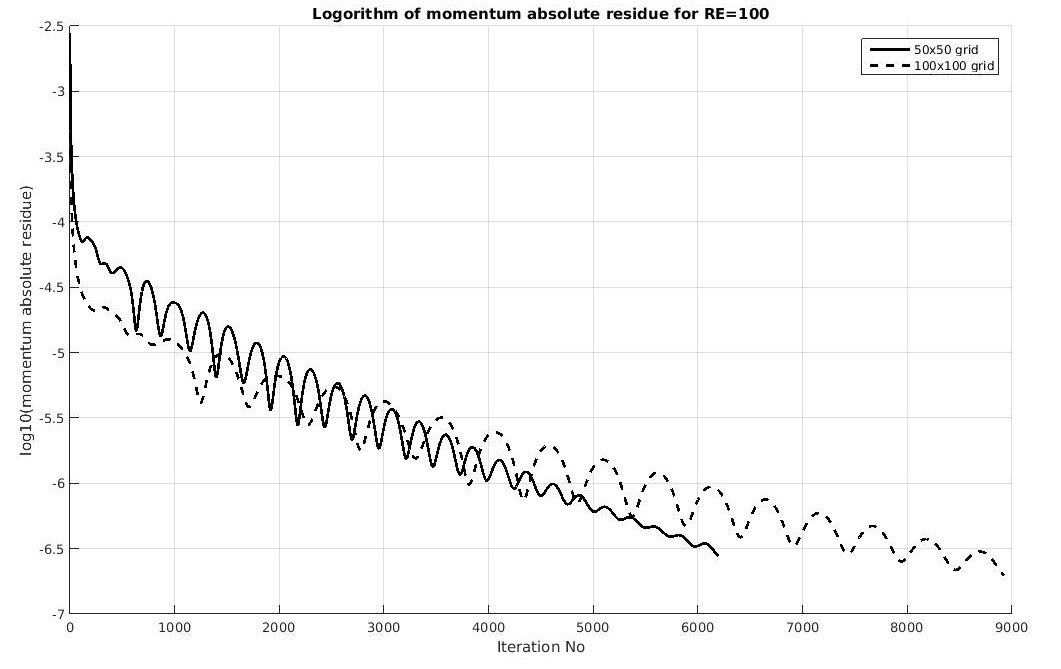
\includegraphics[width=1.0\linewidth]{14_ar_mesh_comparision}
	\end{figure}
	
	\begin{figure}[h]
		\caption{Vorticity contours for Re=100}
		\centering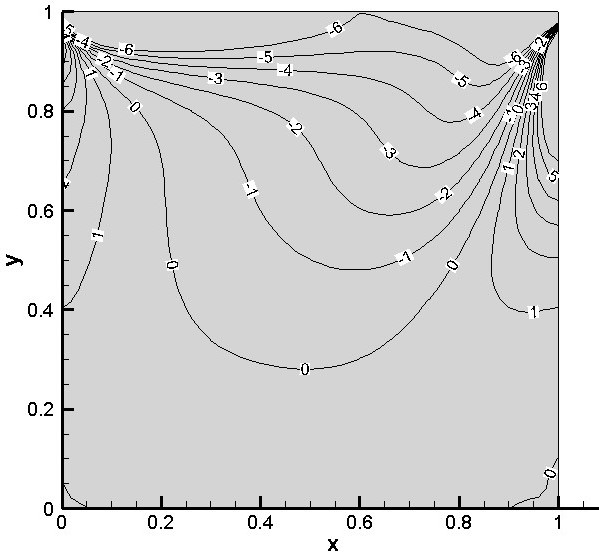
\includegraphics[width=0.8\linewidth]{17_50_50_re_100_TVD_stream_vorticity}
		\caption{Streamlines for Re=100}
		\centering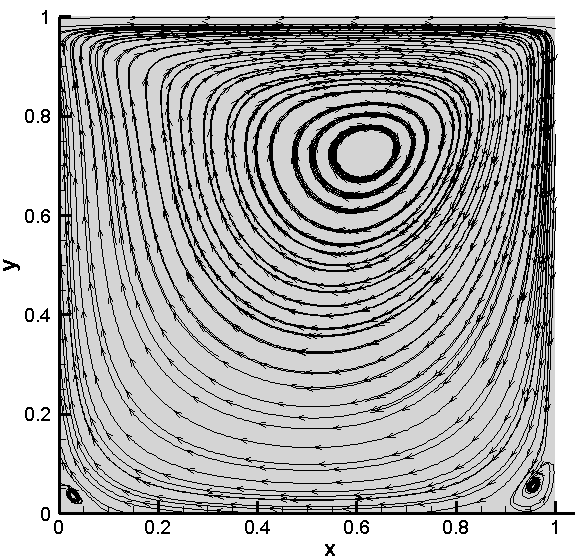
\includegraphics[width=0.8\linewidth]{18_50_50_re_100_TVD_stream}
		\label{End:50x50_RE:100}
	\end{figure}
	\clearpage
	
	Figures. 25- 42 shows the results for Re=250 on grids 50x50 and 100x100 using linear approximation and TVD approximation for Rhi-chow intepretation.\newline
	\newline
	Fig. 25, 26 shows the velocity magnitude contours for linear,  TVD approximation respectively and Fig.27,28 shows the comparison of velocities through geometric centers. It can be observed that there is a difference in the contour profiles and this difference can be observed in the 1d plots. The results using the TVD method significantly improved from the linear approximation case whereas the difference is very small for Re=100. This is because the Reynolds number will increase the inertial forces and so the flow scales decrease. The linear approximation will not be able to capture these small scales and thus TVD method will be more accurate for high Reynolds number flows.  Fig. 29, 30 shows the convergence plot comparing the two methods and it can be observed that the number of iterations to converge using TVD is more than linear approximation as TVD provides a more accurate solution.\newline
	\newline
	Mesh independent study is conducted for Re=250 using a refined mesh 100x 100. Fig. 31 - Fig. 32 shows the velocity magnitude contours and figure 33-34 shows the comparison of u,v velocities along lines through the geometric center. It can be observed that the TVD results are different from linear approximation. By using a 100x100 grid, the difference in velocity values between linear and TVD method is decreasing compared to 50x50. This is because mesh refinement will capture the smaller flow scales and solution using linear approximation will be sufficient to an extent in capturing flow effect at the smaller scales and thus the linear results will be closer to the TVD method. Figures. 35,36 shows the convergence rate comparison for linear and TVD methods. It can be observed that the convergence is rate is similar to the TVD method slightly slower\newline
	\newline
	Fig. 37-38 shows the mesh refinement effect on the flow velocities and Fig 39-40 shows the comparison of convergence plots for 50x50 and 100x100 grids using TVD approximation. It can be observed that the 100x100 mesh is giving better results than the 50x50 grid. Also, the number of iterations required for converging with 100x100 grid is more as the absolute residue is going much lower than 50x50 grid and hence 100x100 grid is more accurate. Fig. 41, 42 shows the vorticity and streamlines respectively. It can be observed that there is recirculation at the bottom right corner of the cavity and the area of recirculation is increased compare to Re=100. This is because the inertial forces will be more compared to viscous forces at a high Reynolds number and the damping will be negligible.
	
	In general, it is observed that TVD approximation improves the accuracy, and the rest of the simulations are conducted using the TVD method for estimating the damping term in mass flux.
	
	\begin{figure}[h]
		\caption{Velocity magnitude with RE=250 and 50x50 grid using linear approximation. }
		\centering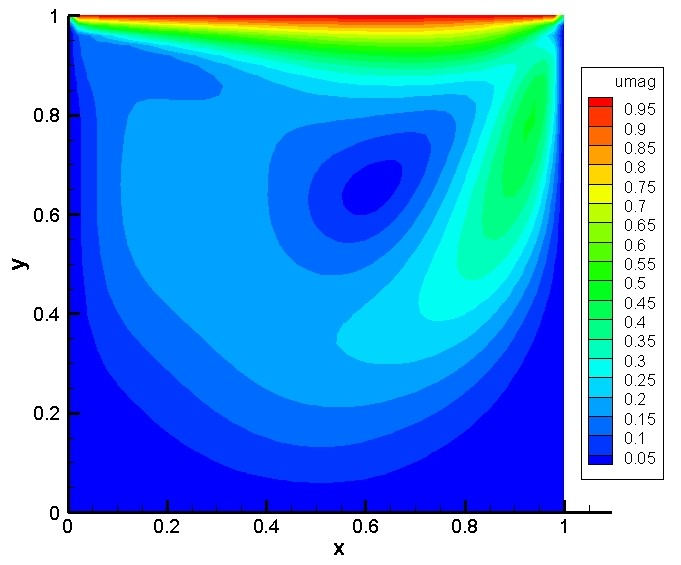
\includegraphics[width=0.9\linewidth]{19_50_50_re_250_velocity_linear}
		\caption{Velocity magnitude with RE=250 and 50x50 grid using TVD method. }
		\centering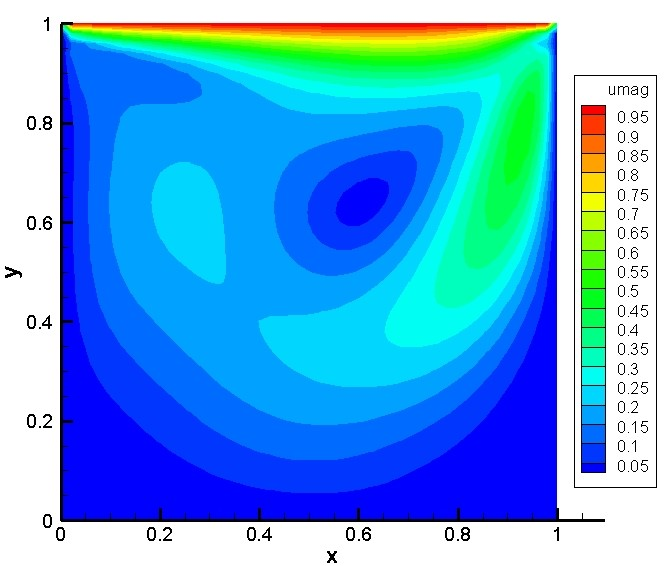
\includegraphics[width=0.9\linewidth]{20_50_50_re_250_velocity_tvd}
	\end{figure}
	
	
	\begin{figure}[h]
		\caption{Comparison of u velocities.}
		\centering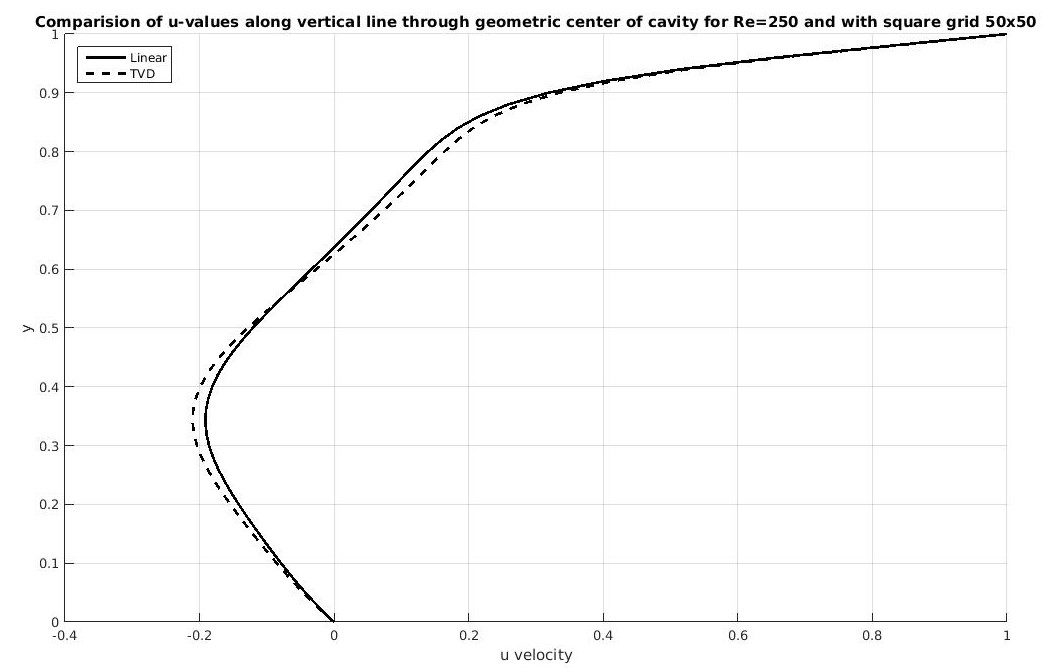
\includegraphics[width=1.0\linewidth]{21_uvalues_tvd_linear_re_250_50_50}
		\caption{Comparison of v velocities.}
		\centering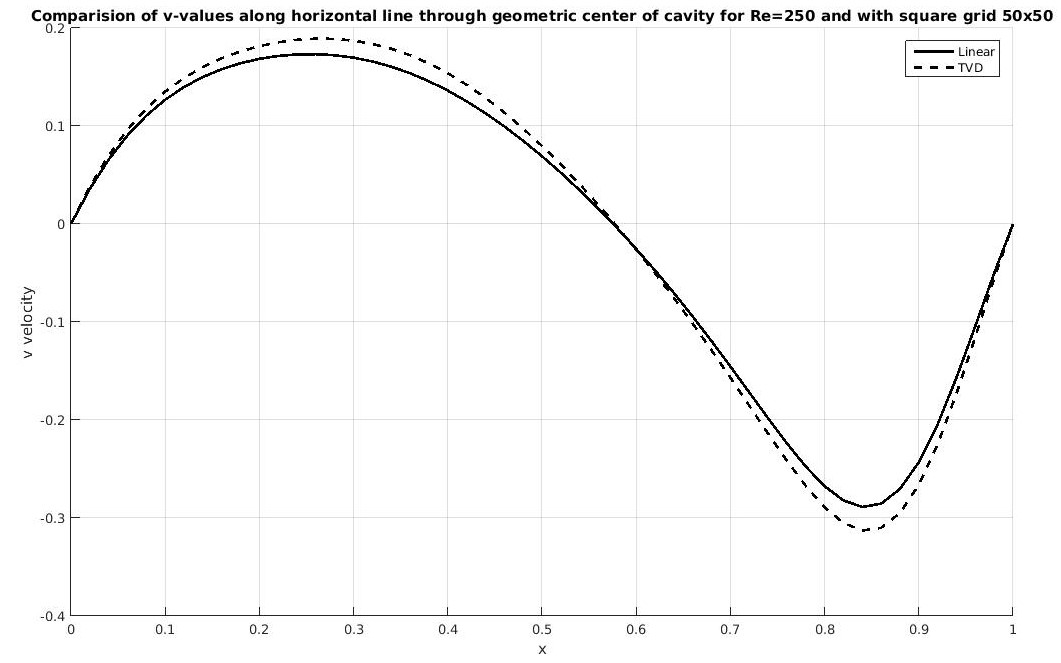
\includegraphics[width=1.0\linewidth]{22_vvalues_tvd_linear_re_250_50_50}
	\end{figure}
	
	\begin{figure}[h]
		\caption{Comparison of Relative Residue.}
		\centering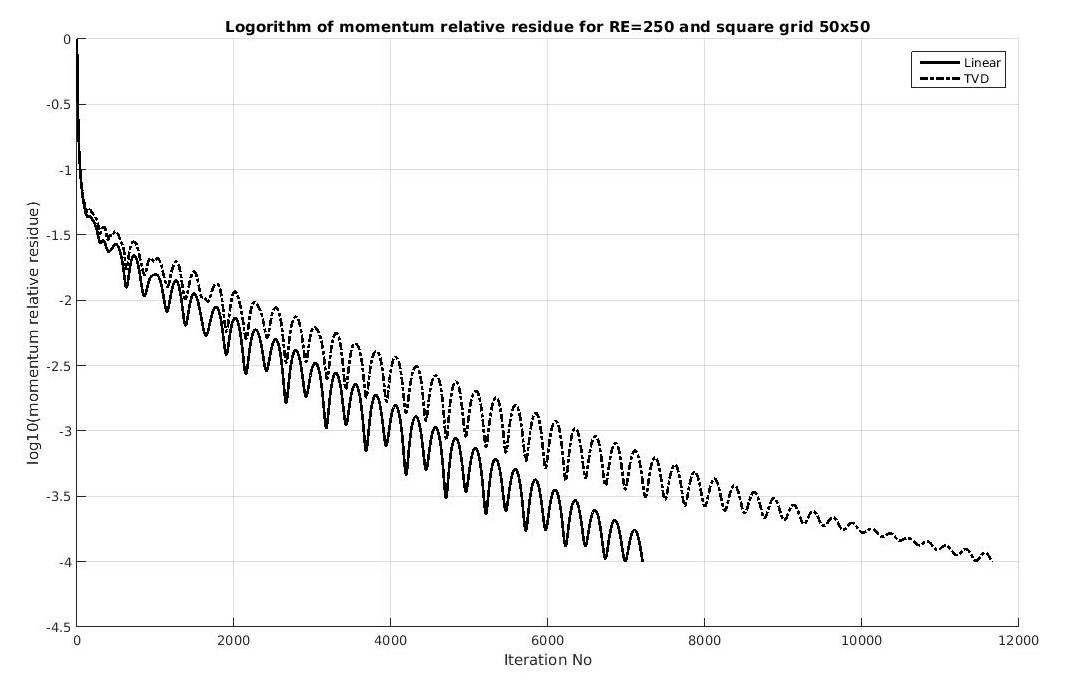
\includegraphics[width=1.0\linewidth]{23_rr_tvd_linear_re_250_50_50}
		\caption{Comparison of Absolute Residue.}
		\centering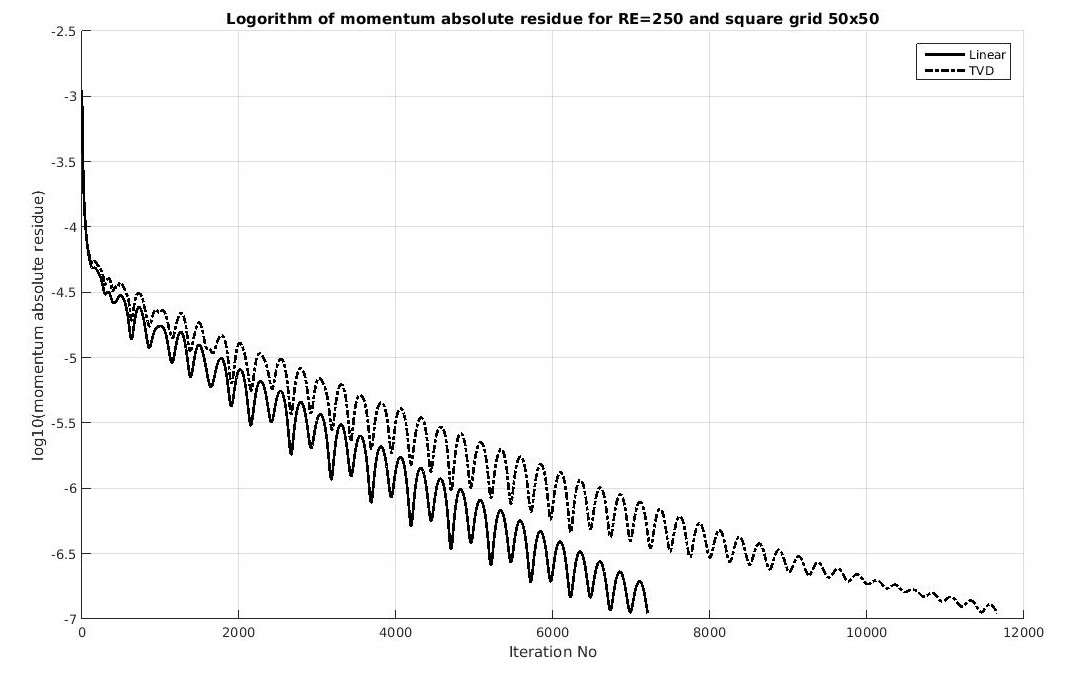
\includegraphics[width=1.0\linewidth]{24_ar_tvd_linear_re_250_50_50}
	\end{figure}
	\clearpage
	
	
	
	
	\begin{figure}[h]
		\caption{Velocity magnitude with RE=250 and 100x100 grid using linear approximation. }
		\centering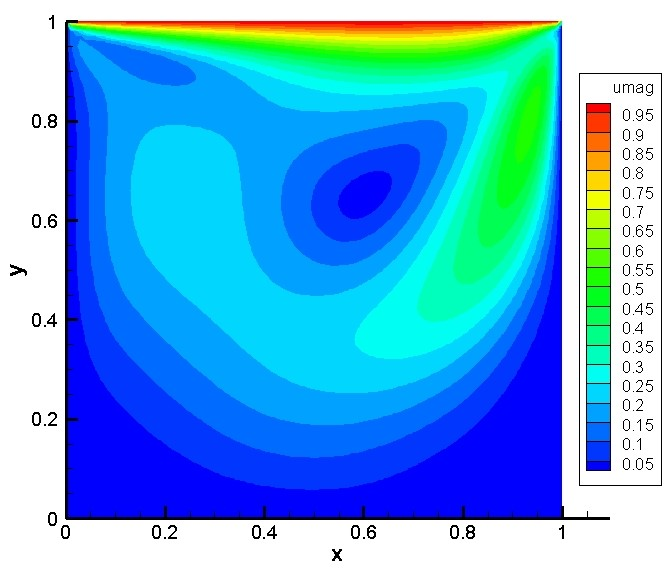
\includegraphics[width=0.9\linewidth]{25_100_100_re_250_velocity_linear}
		\caption{Velocity magnitude with RE=250 and 100x100 grid using TVD approximation. }
		\centering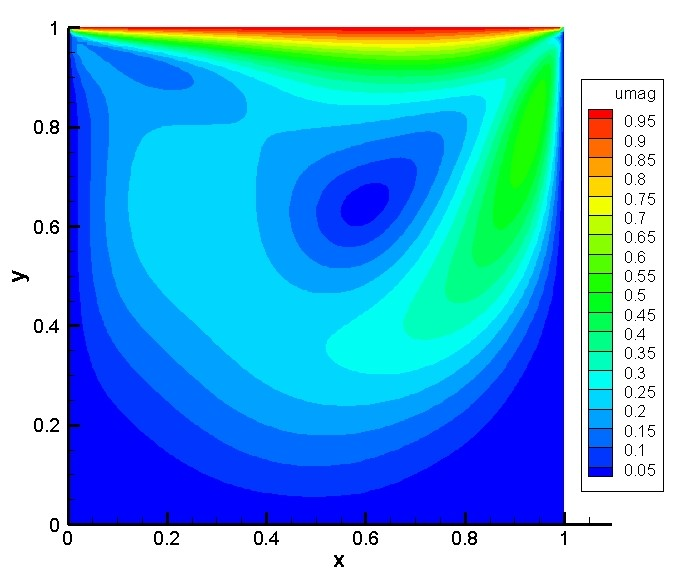
\includegraphics[width=0.9\linewidth]{26_100_100_re_250_velocity_tvd}
	\end{figure}
	
	\begin{figure}[h]
		\caption{Comparison of u velocities.}
		\centering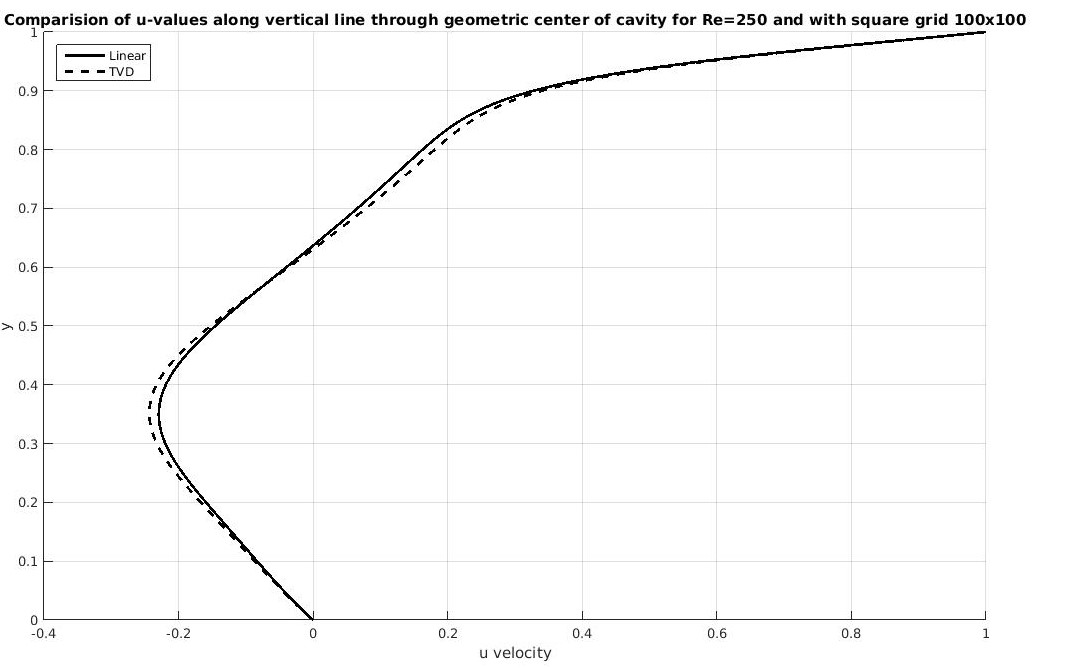
\includegraphics[width=1.0\linewidth]{27_uvalues_tvd_linear_re_250_100_100}
		\caption{Comparison of v velocities.}
		\centering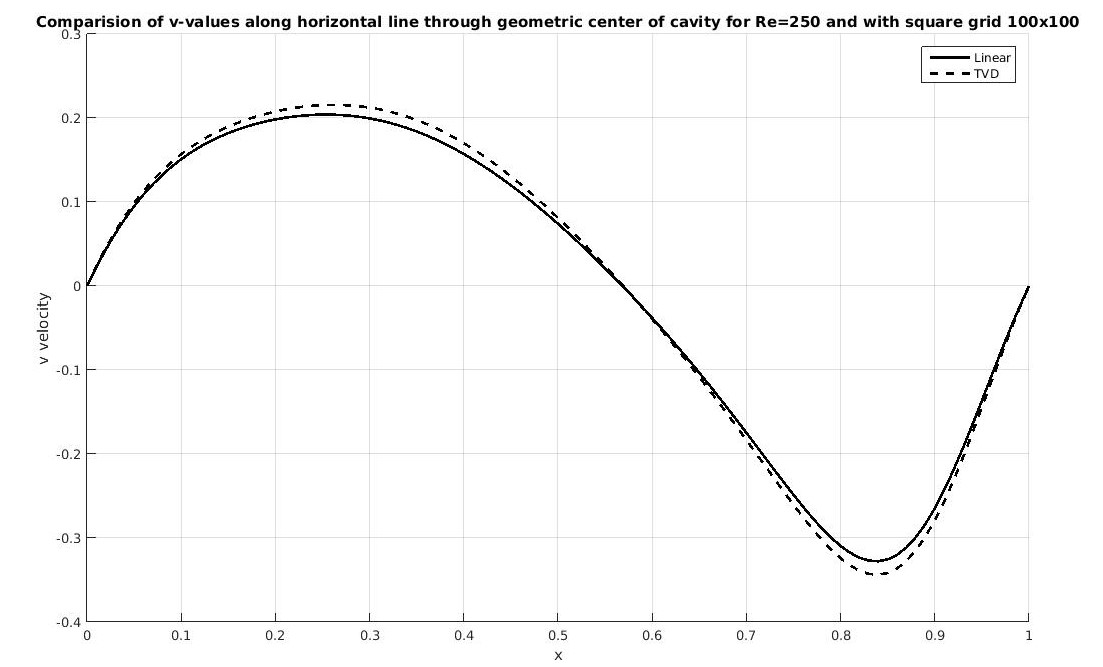
\includegraphics[width=1.0\linewidth]{28_vvalues_tvd_linear_re_250_100_100}
		\label{fig:28_vvalues_tvd_linear_re_250_100_100}
	\end{figure}
	
	\begin{figure}[h]
		\caption{Comparison of Relative Residue.}
		\centering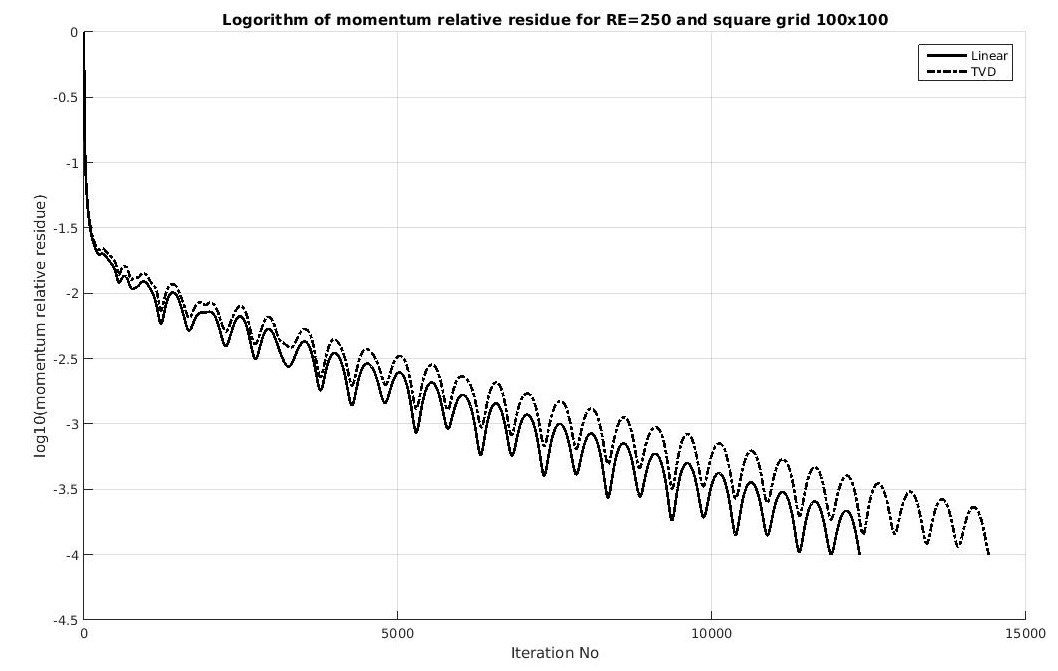
\includegraphics[width=1.0\linewidth]{29_rr_tvd_linear_re_250_100_100}
		\caption{Comparison of Absolute Residue.}
		\centering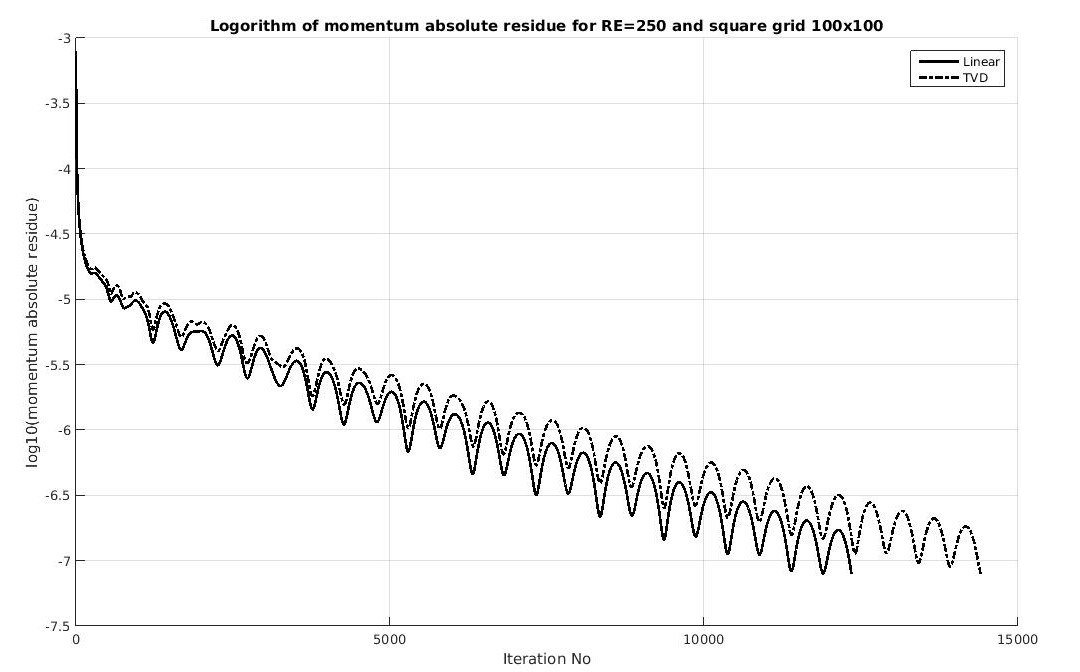
\includegraphics[width=1.0\linewidth]{30_ar_tvd_linear_re_250_100_100}
	\end{figure}
	
	\begin{figure}[h]
		\caption{Comparison of u velocities.}
		\centering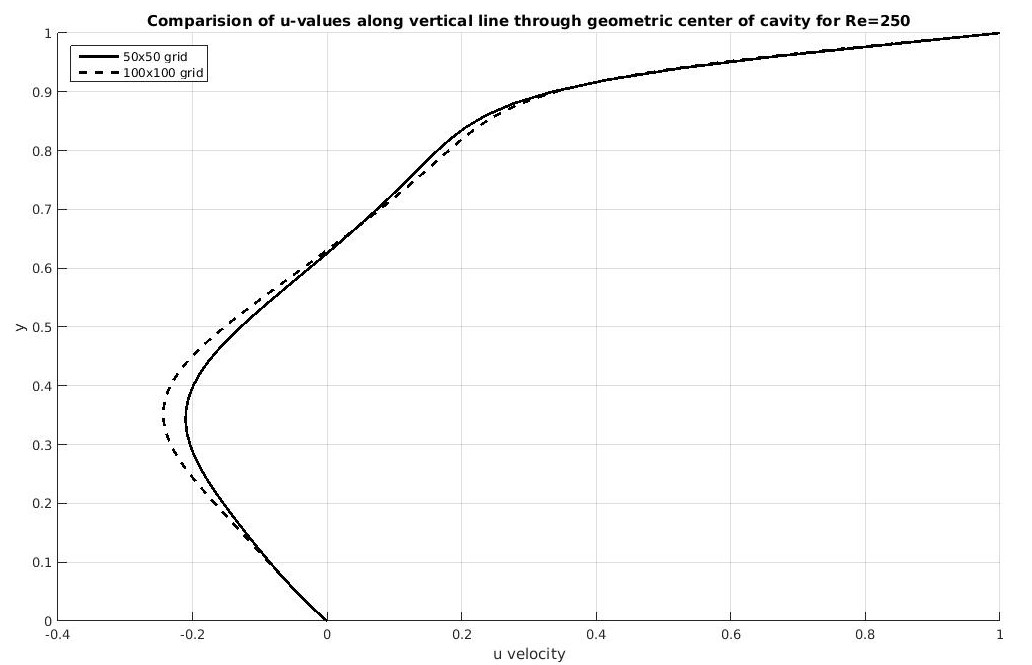
\includegraphics[width=1.0\linewidth]{33_uvel_mesh_re_250_comparision}
		\caption{Comparison of v velocities.}
		\centering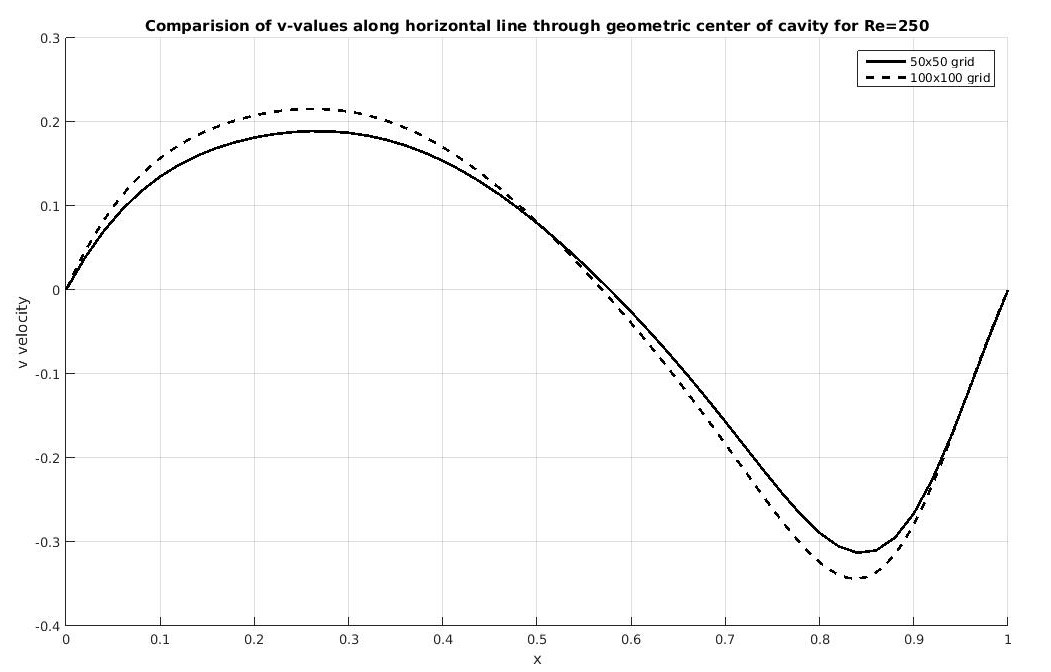
\includegraphics[width=1.0\linewidth]{34_vvel_mesh_re_250_comparision}
	\end{figure}
	
	\begin{figure}[h]
		\caption{Comparison of Relative Residue.}
		\centering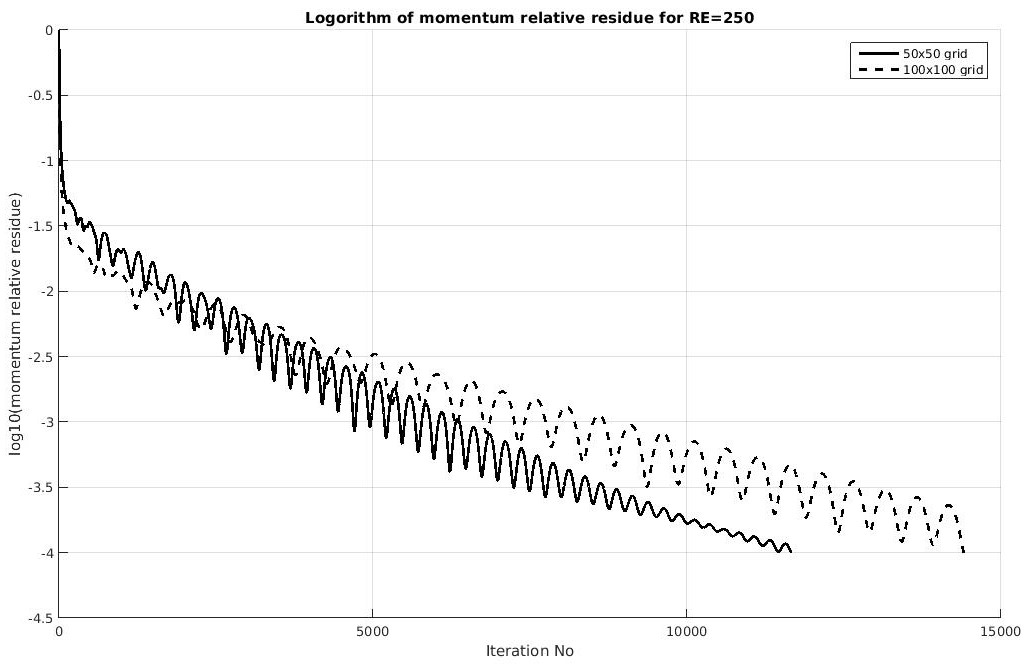
\includegraphics[width=1.0\linewidth]{31_rr_mesh_re_250_comparision}
		\caption{Comparison of Absolute Residue.}
		\centering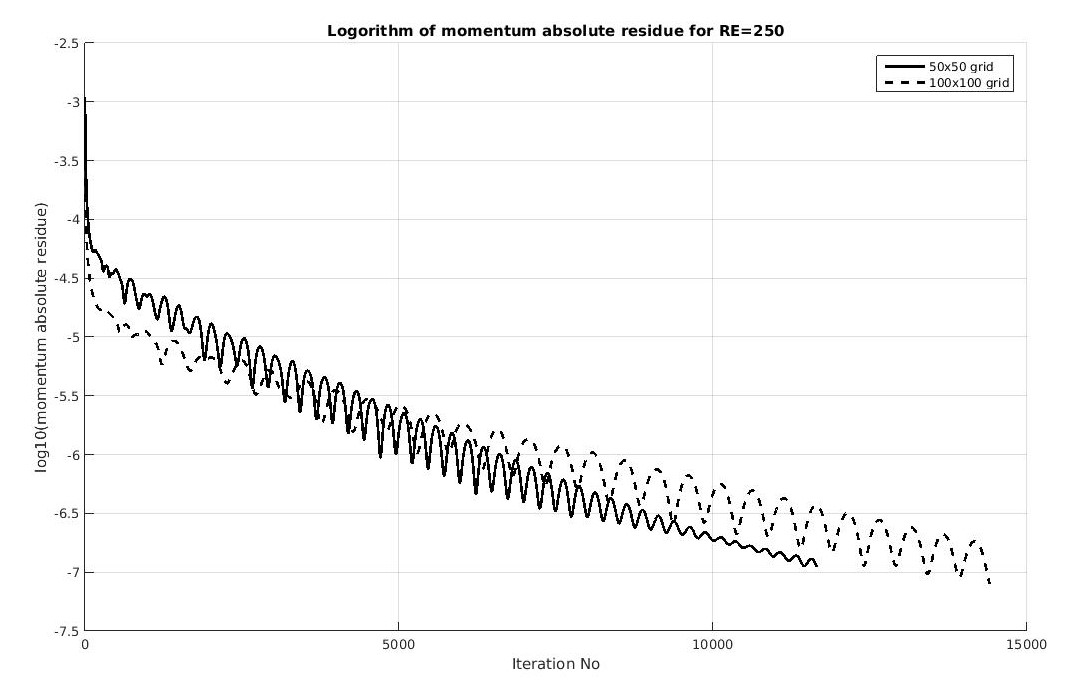
\includegraphics[width=1.0\linewidth]{32_ar_mesh_re_250_comparision}
	\end{figure}
	
	\begin{figure}[h]
		\caption{Streamlines for Re=250}
		\centering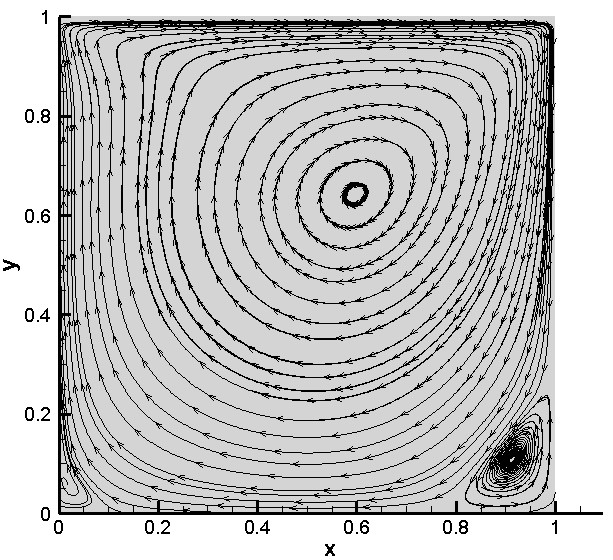
\includegraphics[width=0.8\linewidth]{35_100_100_re_250_streamlines}
		\caption{Vorticity contours for Re=250}
		\centering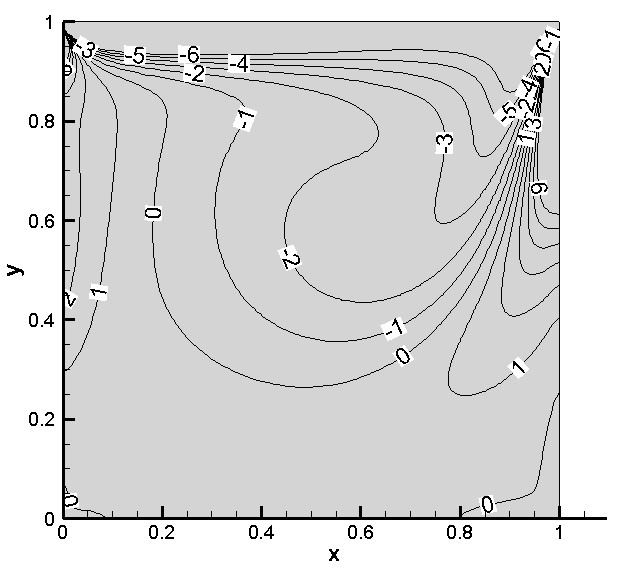
\includegraphics[width=0.8\linewidth]{36_100_100_re_250_vorticity}
	\end{figure}
	\clearpage
	
	The results are also compared with the reference(Ghia et al) for Re=400 and it is observed that the solution using the AC method is deviating by a considerable extent. It can be concluded from this analysis that AC methods are less accurate for high Reynolds numbers. 
	
	\begin{figure}[h]
		\caption{Comparison of u velocities}
		\centering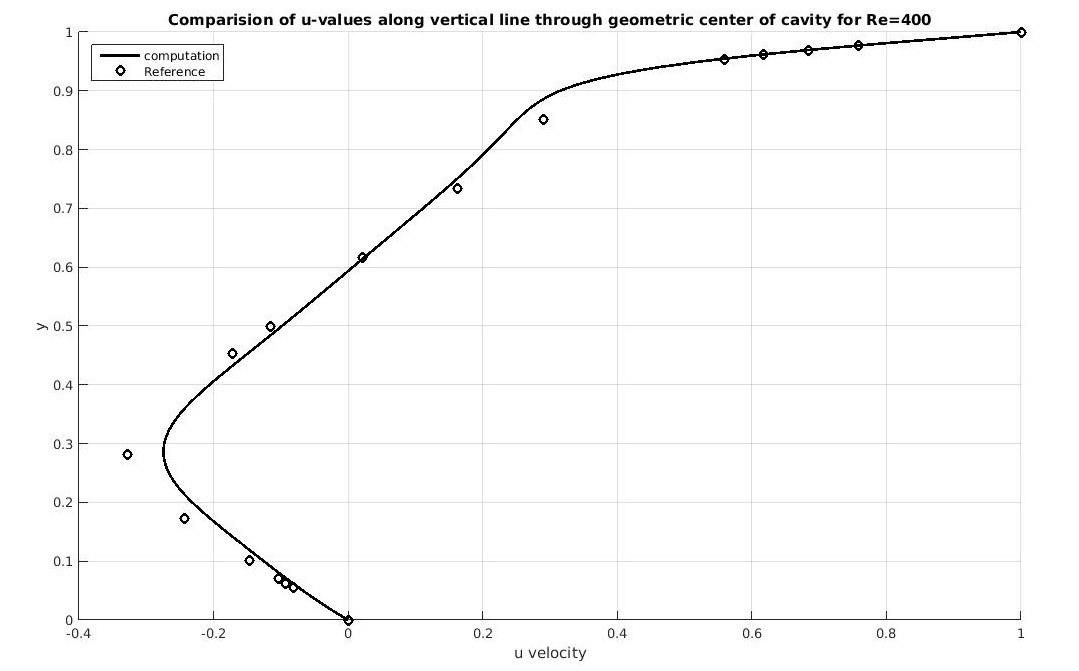
\includegraphics[width=0.7\linewidth]{37_uvel_re_400_comparision}
		\caption{Comparison of v velocities}
		\centering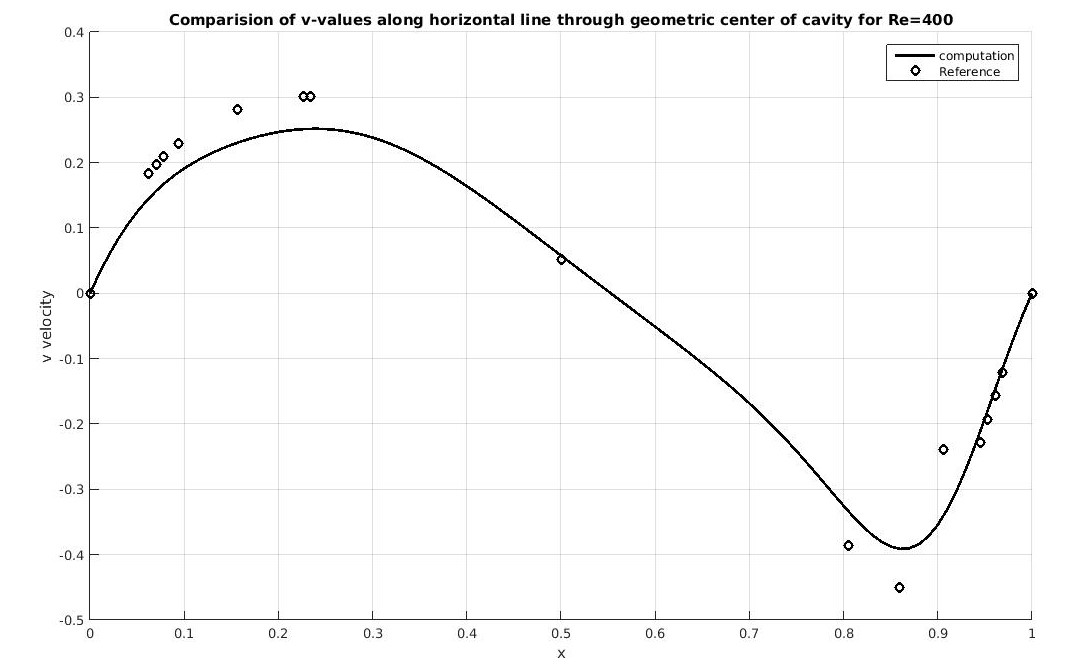
\includegraphics[width=0.7\linewidth]{38_vvel_re_400_comparision}
	\end{figure}
	\clearpage
	
	\subsection{Lid Driven Cavity: Effect of CFL number}
	The code is tested for different kinds of time steps, CFL numbers, and grid sizes on the lid-driven cavity. The local time step is calculated for each cell based on the Eigenvalues and the global time step is the minimum of all the local time steps. Table 1 shows the comparison of results.\newline
	\newline
	The results shows in general that the number of iterations increases with decreasing CFL due to the lower time step. If the case of Re=100 on 50x50 grid is considered, the global time step takes more number of iterations to converge than local time step. This is because of the time step in each cell is less than the locally calculated time step and this will take more number of iterations to reach steady state. Similar trend is observed for cases Re=100, 100x100 and Re=250, 50x50.\newline
	\newline
	\begin{tabular}{ |p{1.0cm}||p{1.7cm}||p{1.7cm}||p{1.7cm}||p{1.7cm}||p{1.7cm}||p{1.7cm}|  }
		\hline
		\multicolumn{7}{|c|}{Table1. Effect of CFL number on reynolds number and mesh refinment} \\
		\hline
		CFL& Re=100 50x50 global& Re=100 50x50 local& Re=100 50x50 global& Re=100 50x50 local& Re=250 50x50 global& Re=250 50x50 local\\
		\hline
		1& 3567& 3132& NC& NC& NC& NC\\
		\hline
		0.9& 3831& 3468& NC& NC& NC& NC\\
		\hline
		0.8& 4288& 3768& NC& NC& NC& NC\\
		\hline
		0.7& 4733& 4155& NC& NC& 9107& NC\\
		\hline
		0.6& 5493& 4674& 7730& NC& 10191& NC\\
		\hline
		0.5& 6367& 5592& 9256& 8235& 11724& 11951\\
		\hline
		0.4& 7908& 6730& 11552& 10252& 14277& 14135\\
		\hline
		0.3& 10201& 8633& 15381& 13630& 18219& 17784\\
		\hline
		0.2& 15176& 12906& 21923& 20389& 26155& 25101\\
		\hline
		0.1& 30070& 24797& 43728& 40668& 49842&	48035\\
		\hline
	\end{tabular}\\
	\newline
	
	The difference in the number of iterations using global and local steps increases with decreasing CFL for all cases. However, this difference in iterations is decreased, for a particular CFL number, if the mesh is refined (Comparing 50x50 grid vs 100x100 grid at Re=100) or the Reynolds number (Comparing 50x50 grid Re=100 vs Re=250) is increased. It is also observed that the simulation did not converge (NC) for certain CFL numbers and the limiting CFL number depends on the grid size, time step criteria, and Reynolds number. It can be observed that the simulation converges even for a higher CFL number if the global time step is used. It is very difficult to predict the cutoff CFL number and to be on the safer side it is better to use a lower CFL number and if convergence issues arise during simulation, the global time step is recommended to use. Fig. 45 shows the comparison of local time step vs global time step for Re=100 and grid size 50x50. It can be observed that the convergence rate using the global time step is slower than the local time step.
	
	\begin{figure}[h]
		\caption{Comparision of convergence plot for local vs global time step using 50x50 grid }
		\centering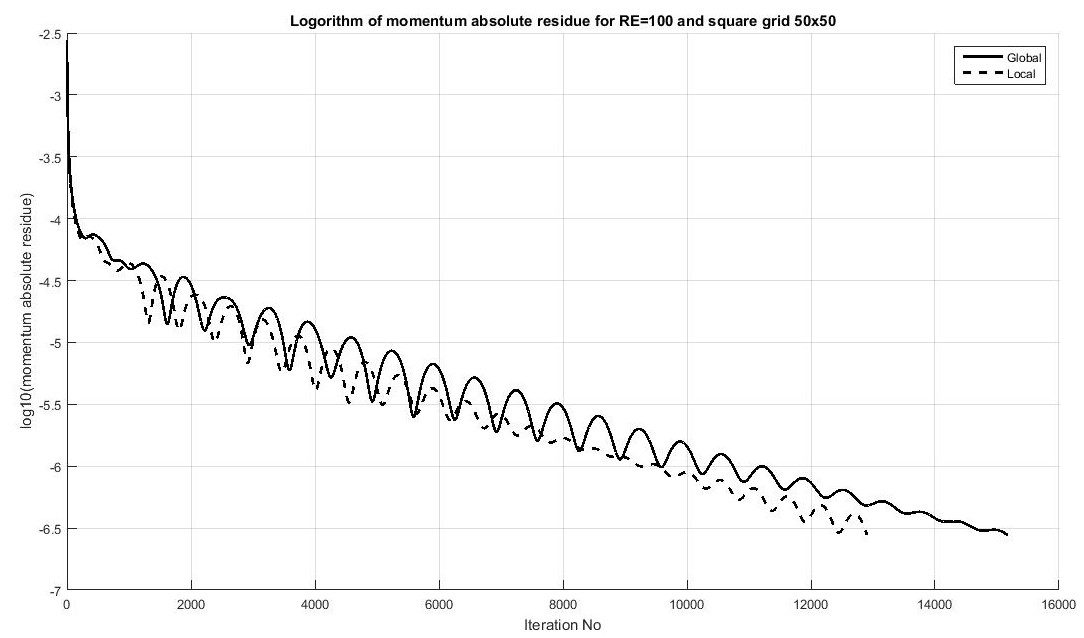
\includegraphics[width=1.0\linewidth]{global_local_ar}
		\centering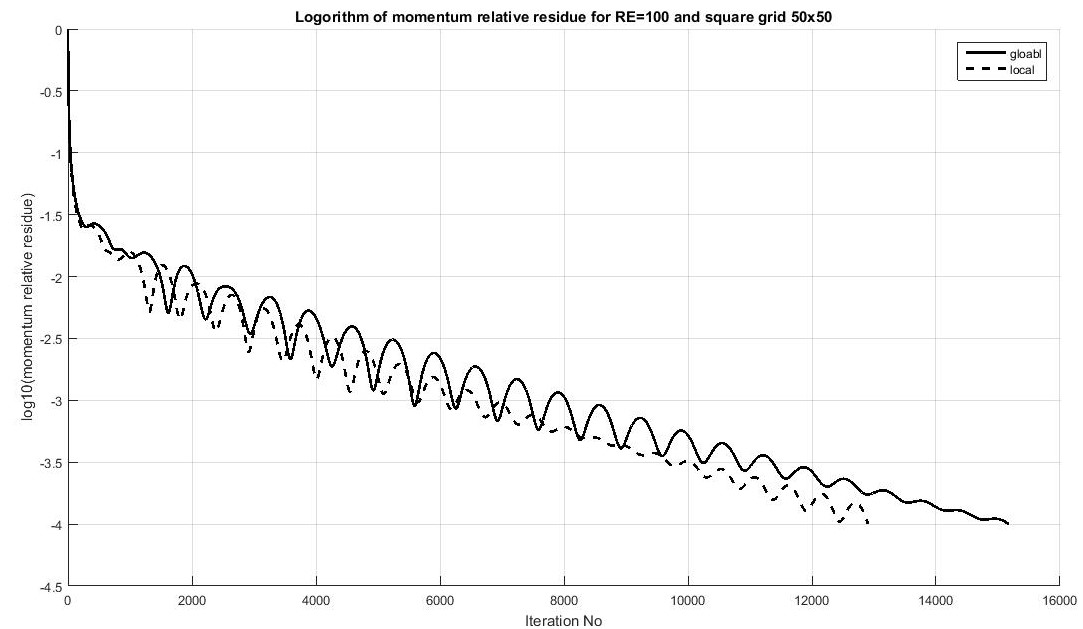
\includegraphics[width=1.0\linewidth]{global_local_rr}
	\end{figure}
	\clearpage
	
	\subsection{Grid 3}
	In this geometry, fully developed flow (with a parabolic profile) enters through the left boundary with a maximum velocity of 1 m/s. The Reynolds number for this problem is defined based on the average inflow velocity (2/3*Umax) and channel height at the inlet. The model is simulated using CFL=0.2 and using TVD approximation. A tolerance of 1e-4 is used for both mass and momentum residue for the convergence criteria. Figure 46-54 are the results for grid3. Fig.46 and Fig.47 show the velocity magnitude for Re=100 and Re=250 respectively. The results show that the circulation region is increasing with an increase in Reynolds number and the flow reattaches at the farthest point. This can be confirmed by the streamlined plot shown in Fig. 48 and 49. The reason for larger circulation is because the inertial forces are more compared to viscous forces at high Reynolds and the flow tends to follow its path for a long distance before bending.\newline
	\newline
	Fig. 50-51 and Fig. 52-53 show the convergence plot for Re=100 and Re=250 respectively. The solver terminates when the relative residue is 1e-4 in both mass, momentum. It can be observed that mass residue goes below the tolerance at a certain point of the simulation but the solver is not converged as momentum residue doesn’t go below tolerance. It can be also observed that the convergence rate is slower for Re=250 than Re=100. This is because local time steps will be small as the flow scales are small at a higher Reynolds number. Fig.54 shows the convergence plot for TVD vs linear and it is observed that both converges in a similar trend.
	
	\begin{figure}[h]
		\caption{Velocity Magnitude contours for Re=100}
		\centering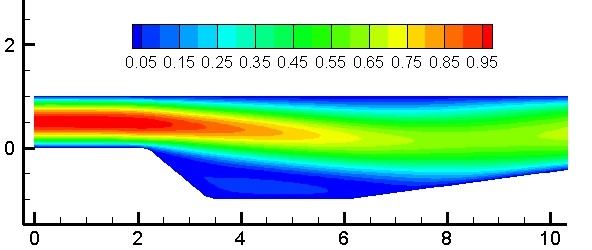
\includegraphics[width=0.7\linewidth]{43_grid3_umag_100}
		\caption{Velocity Magnitude contours for Re=250}
		\centering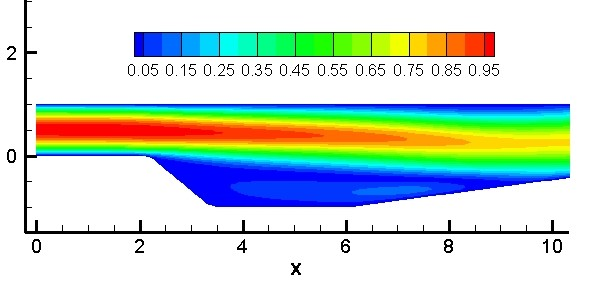
\includegraphics[width=0.7\linewidth]{44_grid3_umag_re_250}
		\caption{Streamlines for Re=100}
		\centering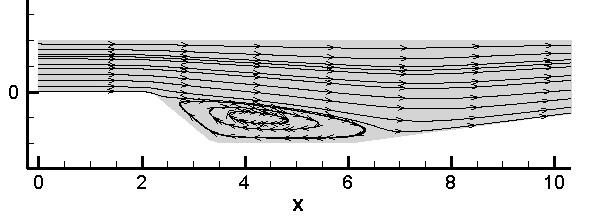
\includegraphics[width=0.7\linewidth]{45_grid3_streamlines_100}
		\caption{streamlines for Re=250}
		\centering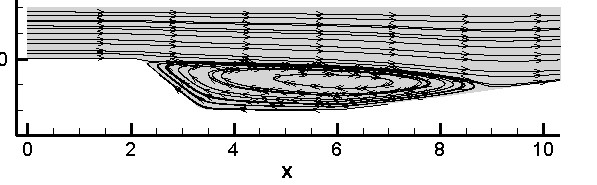
\includegraphics[width=0.7\linewidth]{46_grid3_streamlines_250}
	\end{figure}
	
	
	\begin{figure}[h]
		\caption{Convergence plot}
		\centering\includegraphics[width=1.0\linewidth]{51_grid3_rr_re_100}
		\caption{Convergence plot}
		\centering\includegraphics[width=1.0\linewidth]{52_grid3_ar_re_100}
	\end{figure}
	
	\begin{figure}[h]
		\caption{Convergence plot}
		\centering\includegraphics[width=1.0\linewidth]{53_grid3_rr_re_250}
		\caption{Convergence plot}
		\centering\includegraphics[width=1.0\linewidth]{54_grid3_ar_re_250}
	\end{figure}
	
	\begin{figure}[htbp]
		\caption{Comparision of convergence plot for grid3 Re=100}
		\centering\includegraphics[width=1.0\linewidth]{grid3_rr_comparision}
		\centering\includegraphics[width=1.0\linewidth]{grid3_ar_comparision}
	\end{figure}
	
	
	\clearpage
	\subsection{Grid4}
	Simulation is also conducted on grid 4 to capture the flow. The flow structure follows a similar trend as that of grid3 like the circulation area increases with Reynolds number. 
	
	\begin{figure}[h]
		\caption{Velocity Magnitude contours for Re=100 on Grid 4}
		\centering\includegraphics[width=0.7\linewidth]{48_grid4_streamlines_100}
		\caption{Velocity Magnitude contours for Re=250 on Grid 4}
		\centering\includegraphics[width=0.7\linewidth]{49_grid4_streamlines_250}
		\caption{Streamlines for Re=100 on Grid 4}
		\centering\includegraphics[width=0.7\linewidth]{47_grid4_streamlines_100}
		\caption{streamlines for Re=250 on Grid 4}
		\centering\includegraphics[width=0.7\linewidth]{50_grid4_streamlines_250}
	\end{figure}
	
	\clearpage
	
	\subsection{Immerssed boundary simulation}
	The AC incompressible method for solving the Naiver Stokes equation is extended to include the immersed boundary technique for steady flows. The code is tested with various types of geometries. The first problem is a  flow past a cylinder of diameter 0.1 m with fully developed flow condition at the inlet and with a maximum velocity of 1. The Reynolds number of the problem is 25 and it is well below the critical Reynolds for the flow to be unstable. Fig. 59-62 are the results for the problem and it can be observed that the streamlines are well captured by the immersed boundary method.\newline
	\newline
	In the second problem, an additional object is used along with cylinder the detection capability of IB. Fig 63-65 are the results for the problem and it can be observed that the circulations are captured in the simulation.\newline
	\newline
	In the third problem, two cylinders of radius 0.125 is placed in the circulation region of grid4, and flow is captured around the two cylinders. The Reynolds number used for the problem is 100. Fig. 66 and 67 show the domain and velocity magnitude distribution for the problem\newline
	\newline
	In the fourth problem, two cylinders are placed in a lid-driven cavity, and flow around the cylinders in the cavity is modeled. The radius of the cylinders is 0.1 each and a Reynolds number of 100 is used for the simulation. For this problem, a square grid of 200x200 elements is used. Fig. 68- 70 shows the domain and velocity magnitude distribution for the problem.\newline
	\newline
	In the fifth problem, the complexity is slightly increased by using five cylinders of 0.2 m diameter, and the square cavity of 2m x 2m  is used with 200x200 mesh elements. The Reynolds for the problem based on cavity length is 200. Fig. 71- 73 shows the domain and velocity magnitude distribution for the problem.\
	
	\begin{figure}[h]
		\caption{Domain 1}
		\centering\includegraphics[width=0.7\linewidth]{55_immerssed_boundary_cylinder_domain}
		\caption{Velocity Magnitude contours for Re=25 based on cylinder diameter}
		\centering\includegraphics[width=0.7\linewidth]{55_immerssed_boundary_cylinder}
		\caption{Streamlines for for Re=25 based on cylinder diameter}
		\centering\includegraphics[width=0.7\linewidth]{55_immerssed_boundary_cylinder_streamlines}
		\caption{streamlines for for Re=25 based on cylinder diameter}
		\centering\includegraphics[width=0.7\linewidth]{55_immerssed_boundary_cylinder_streamlines_zoomed}
	\end{figure}
	
	\begin{figure}[h]
		\caption{Domain 2}
		\centering\includegraphics[width=0.7\linewidth]{57_immerssed_boundary_umag_domain}
		\caption{Velocity Magnitude distribution for Re=266 based on channel inlet length}
		\centering\includegraphics[width=0.7\linewidth]{57_immerssed_boundary_umag}
		\caption{Streamlines for Re=266 based on channel inlet length}
		\centering\includegraphics[width=0.7\linewidth]{57_immerssed_boundary_streamilnes}
	\end{figure}
	
	\begin{figure}[h]
		\caption{Domain 3}
		\centering\includegraphics[width=0.7\linewidth]{56_immerssed_boundary_domain}
		\caption{Velocity Magnitude distribution for Re=100 based on channel inlet length}
		\centering\includegraphics[width=0.7\linewidth]{56_immerssed_boundary_umag}
	\end{figure}
	
	\begin{figure}[h]
		\caption{Domain 4}
		\centering\includegraphics[width=0.7\linewidth]{58_immerssed_boundary_domain}
		\caption{Velocity Magnitude distribution for Re=100 based on cavity length}
		\centering\includegraphics[width=0.7\linewidth]{58_immerssed_boundary_umag}
	\end{figure}
	
	\begin{figure}[h]
		\caption{Streamlines for Re=100 based on cavity length}
		\centering\includegraphics[width=0.7\linewidth]{58_immerssed_boundary_streamlines}
		\caption{Domain 5}
		\centering\includegraphics[width=0.7\linewidth]{59_immerssed_boundary_umag}
	\end{figure}
	
	\begin{figure}[h]
		\caption{Velocity Magnitude distribution for Re=100 based on cavity length}
		\centering\includegraphics[width=0.7\linewidth]{59_immerssed_boundary_velocity}
		\caption{Streamlines for Re=100 based on cavity length}
		\centering\includegraphics[width=0.7\linewidth]{59_immerssed_boundary_streamlines}
	\end{figure}
	\clearpage
	
	\section{Appendix}
	\label{S:2}
	
	\bibliographystyle{model1-num-names}
	\bibliography{sample.bib}
	
	
\end{document}
